\documentclass[12pt,bibliography=oldstyle,DIV=12,parskip=half-]{scrreprt}


\iflatexml
% \documentclass[12pt,bibliography=oldstyle,DIV=12,parskip=half-]{scrreprt} % Not (yet) supported by LaTeXML.
\fi

\include{conf/preconfig}
\include{conf/packages}
\include{conf/config}
\include{conf/comandos}
\include{conf/fuentes}
% First macro on next line not (yet) supported by LaTeXML: 
% \addbibresource{res/bibliografia.bib}
\hyphenation{micro-RNA}
\hyphenation{micro-RNAs}
\hyphenation{mi-RNA}
\hyphenation{mi-RNAs}
% First macro on next line not (yet) supported by LaTeXML: 
% \addtokomafont{descriptionlabel}{\small}
% First macro on next line not (yet) supported by LaTeXML: 
% \setkomafont{subject}{\LARGE\usekomafont{disposition}}
% First macro on next line not (yet) supported by LaTeXML: 
% \setkomafont{title}{\normalfont\slshape}
% First macro on next line not (yet) supported by LaTeXML: 
% \setkomafont{subtitle}{\LARGE\usekomafont{disposition}}
\setlength{\abovecaptionskip}{-10pt plus 3pt minus 2pt}
\setlength{\belowcaptionskip}{10pt plus 3pt minus 2pt}
\hypersetup{
  colorlinks,
  citecolor=black,
  filecolor=black,
  linkcolor=black,
  urlcolor=black
}
% First macro on next line not (yet) supported by LaTeXML: 
% \sisetup{
%  table-number-alignment = right,
%  group-separator = ,
%  output-decimal-marker = {,},
%  retain-explicit-plus = true
%}
\newcommand{\e}[][]{\emph}

\newcommand{\fr}[1][]{(\autoref{#1})}

\newcommand{\iid}[][]{independiente e idénticamente distribuido}

\newtheorem{definicion}{Definición}[chapter]
\newtheorem{lema}[definicion]{Lema}
\newcommand{\ntA}[][]{\textrm{\mono{A}}{ }}

\newcommand{\ntC}[][]{\textrm{\mono{C}}{ }}

\newcommand{\ntG}[][]{\textrm{\mono{G}}{ }}

\newcommand{\ntU}[][]{\textrm{\mono{U}}{ }}

\newcommand{\pairL}[][]{\textrm{\mono{(}}{ }}

\newcommand{\pairR}[][]{\textrm{\mono{)}}{ }}

\newcommand{\noPair}[][]{\textrm{\mono{.}}{ }}

\newcommand{\dn}[1][]{\textrm{\mono{#1}}{ }}

\newcommand{\bp}[2][]{\textrm{\mono{#1-#2}}{ }}

\newcommand{\grad}[1][]{\nabla{#1}}

\newcommand{\tableStyle}[][]{\relsize{-0.5}\center\sffamily}

\newcommand{\captionStyle}[][]{\relsize{-0.5}}

\newcommand{\tE}[][]{&{\smaller $\bar{x}$}&}

\newcommand{\tF}[1][]{\multirow{2}{*}{#1}\tE}

\newcommand{\tZ}[][]{&{\smaller $\sigma$}&}

\newcommand{\tA}[][]{\addlinespace[4pt]}

\newcommand{\rowMEAN}[1][]{&\multirow{2}{*}{#1}&{\smaller $\bar{x}$}}

\newcommand{\rowSTD}[][]{&&{\smaller $\sigma$}}

\newcommand{\rowSKIP}[][]{\addlinespace[2pt]}

\newcommand{\ti}[][]{\textsmaller}

\newcommand{\func}[1][]{\emph{#1}}

\newcommand{\Gm}[][]{\scriptsize $G_m$}

\newcommand{\Ft}[1][]{\mrow{2}{*}{#1}}

\newcommand{\tbmean}[][]{\smaller{2} $\bar{x}$}

\newcommand{\tbstd}[][]{\smaller $\sigma$}

\newcommand{\tripletsvm}[][]{\sbsf{Triplet-SVM}}

\newcommand{\mipred}[][]{\sbsf{miPred}}

\newcommand{\micropred}[][]{\sbsf{microPred}}

\newcommand{\deltamirbase}[][]{\sbsf{$\mathbf{\mathsf{\Delta}}$miRBase}}

\newcommand{\rowMEANN}[2][]{&
  \multirow{2}{*}{\tablenum[table-format=1.0,table-number-alignment=right]{#1}}&
  \multirow{2}{*}{\tablenum[table-format=3.0,table-number-alignment=right]{#2}}&
           {\smaller $\bar{x}$}}

\newcommand{\rowSTDN}[][]{&&&{\smaller $\sigma$}}

% First macro on next line not (yet) supported by LaTeXML: 
% \DeclareSIUnit\nt{nt}
\newcommand{\VP}[][]{\T{\textsl{VP}}}
\newcommand{\VN}[][]{\T{\textsl{VN}}}
\newcommand{\FP}[][]{\T{\textsl{FP}}}
\newcommand{\FN}[][]{\T{\textsl{FN}}}
\newcommand{\SE}[][]{\T{\textsl{SE}}}
\newcommand{\SP}[][]{\T{\textsl{SP}}}
\newcommand{\GM}[][]{\T{\textsl{Gm}}}
\newcommand{\PR}[][]{\T{\textsl{Pr}}}
\newcommand{\AC}[][]{\T{\textsl{Ac}}}
\newcommand{\feedforward}[][]{con propagación hacia adelante}
\newcommand{\headRow}[][]{  \sfbf{\footnotesize Pos.} &
  \sfbf{\footnotesize Característica} &
  \sfbf{\footnotesize Descripción}
}
\newcommand{\tripletRow}[1][]{
  \stepcounter{FeatureCounter}\theFeatureCounter & $N_{\T{\mono{#1}}}$
  & Ocurrencias del triplete \mono{#1} en la región del tallo.}
\newcommand{\dnRow}[1][]{
  \stepcounter{FeatureCounter}\theFeatureCounter & $N_{\T{\mono{#1}}}$
  & Número de dinucleótidos \mono{#1} en la secuencia.}
\newcommand{\funcheader}[3][]{\begin{description}%
  \item[Función]{#1}\item[Entradas]{#2}\item[Salidas]{#3}%
\end{description}}
\renewcommand{\bibfont}[][]{\normalfont\footnotesize}

\iflatexml\else\ohead{\small capitulo3-tmp, rev. 2e32658+, \today}\fi

\begin{document}
\selectlanguage{spanish}
\title{Informe Final - Capítulo 3}

%
\begin{abstract}
%
DevOps es un conjunto de prácticas y principios utilizados para
agilizar la producción del software. Busca generar una cultura en
común dentro de las organizaciones integrando el trabajo de las
diferentes áreas involucradas en la producción y entrega del
software. Propone aprovechar la automatización para eliminar trabajo
innecesario de las personas, y destaca la importancia de establecer un
proceso de mejora continua basado en objetivos medibles y
verificables.
  
En este Proyecto se implementaron prácticas y herramientas
tecnológicas en busca de integrar el trabajo de desarrollo y
operaciones de acuerdo a la propuesta DevOps. El trabajo incluyó la
automatización de tareas de infraestructura, la implementación de
tuberías de integración y entrega continuas y la unificación de los
repositorios de código fuente y configuración. Asimismo, se
implementaron herramientas para brindar autoservicio de la
infraestructura, visibilidad de métricas y registros y
comunicación. El ámbito de trabajo fue la Dirección de Informatización
y Planificación Tecnológica de la Universidad Nacional del Litoral
(DIPT-UNL).
%
\end{abstract}
%

\titlehead{\center\large
\includegraphics[width=4cm]{figures/logofichunl/logofichunl.pdf}\smallskip\\
 Universidad Nacional del Litoral\\
 Facultad de Ingeniería y Ciencias Hídricas
}

\subject{
 Proyecto Final de Carrera\\
 Ingeniería en Informática
}
\subtitle{
}

\publishers{
}

\date{\today}

\author{  Alumno: Mauro J. Torrez\\
  Directora: Ing. Claudia S. Arrietti
}

\dedication{\normalfont\normalsize\itshape
A mis padres, gracias a su esfuerzo y apoyo hoy estoy aquí.

A mis hermanos y a mis amigos, quienes me acompañaron durante todo
este tiempo.

A mi directora, por la confianza en este proyecto.

A mi madrina, por alentarme siempre a trabajar para alcanzar este
objetivo.

A mi abuela Nydia, quien hubiera sido la persona más orgullosa de este
logro.
}

\renewcommand*{\titlepagestyle}{empty}
\maketitle

%
%
%
%
\iflatexml{}\else\setcounter{chapter}{2}\fi%
%
\chapter{Descripción del método}
%
El método desarrollado es en un sistema completo de reconocimiento de
\premirna{s}, con funcionalidad para la generación de un modelo de
clasificador y para su aplicación posterior sobre nuevos datos.

Como punto de partida se consideraron los trabajos
\cite{xue,ng,batuwita,sheng,sewer,ding}, en los que se presentan
herramientas de software con propósito similar al del presente
desarrollo.
En particular, debido a la disponibilidad de datos suplementarios,
se utilizaron los conjuntos de datos y se implementaron técnicas de
extracción de \caract{s} de los trabajos \cite{xue,ng,batuwita}.

La implementación se efectuó en lenguaje Matlab versión R2012b,
haciendo uso uso de los módulos adicionales ``Neural Network Toolbox''
y ``Bioinformatics Toolbox''.
Además, se integraron las herramientas de software \work{libSVM}
\cite{libsvm} y \work{RNAFold} \cite{vienna}.
Se utilizó el software \work\webdemo{} \cite{webdemobuilder} para
la creación de la interfaz web.

%
%
%
\section{Descripción general}
%
La arquitectura del software codificado se describe en torno a
tres componentes principales: \e{preprocesamiento}, \e{generación
del modelo del clasificador}, y \e{clasificación}. 

El preprocesamiento transforma los datos de entrada desde su forma
original de cadenas de caracteres a un formato numérico tratable por
la máquina de aprendizaje.
Abarca la lectura e interpretación de los archivos de entrada, la
extracción de \caract{s}, y otras tareas de preparación de los datos,
generando una representación interna de los datos que se utiliza como
entrada a la máquina de aprendizaje, ya sea para la generación del
modelo o para clasificación.

La generación del modelo del clasificador aplica estrategias de
selección de \hparam{s} y efectúa el entrenamiento
para obtener un modelo de clasificador óptimo.
Como entrada, recibe los datos del preprocesamiento y procede en dos
pasos: en primer lugar, aplica alguna estrategia para determinar los
hiperparámetros óptimos, y luego efectúa el entrenamiento propiamente
dicho.
A la salida devuelve un modelo de clasificador que puede ser
utilizado para la predicción de clase de nuevas secuencias.

La clasificación obtiene predicciones de clase sobre nuevos ejemplos
aplicando un modelo generado previamente.
Para la obtención de predicciones de clase, se debe contar con un
modelo de clasificador generado previamente, además de archivos de
secuencias para clasificar.
El primer paso es aplicar el preprocesamiento sobre los archivos de
entrada, generando un conjunto de datos denominado ``de prueba''.
Luego se aplica el modelo sobre este conjunto, obteniendo a la salida
las predicciones de clase correspondientes.

%% El preprocesamiento lee a su entrada archivos en un formato de texto
%% estándar denominado FASTA, y aplicando un proceso denominado
%% extracción de características, convierte los datos leídos a matrices
%% numéricas.
%% Los datos numéricos son luego reagrupados en nuevas matrices que
%% representan los conjuntos de datos utilizados por la máquina de
%% aprendizaje.

%% Cuando el objetivo es la generación de un modelo de clasificador, la
%% entrada al sistema consiste en archivos de texto con secuencias de
%% ejemplo.
%% Por cada archivo, se especifica una clase, indicando que el mismo
%% contiene ejemplos de \premirna{s} validados (clase positiva) o bien
%% ejemplos de ``pseudo'' \premirna{s} (clase negativa).
%% Se requiere la especificación de al menos un archivo de cada clase.
%% Aplicando preprocesamiento, estos archivos se utilizan para el armado
%% del conjunto de entrenamiento.

%
%
%
\section{Preprocesamiento}
%
El preprocesamiento se encarga de transformar los datos de entrada,
que vienen dados en forma de archivos de texto, a un formato numérico
apto para la máquina de aprendizaje.
Los pasos efectuados en la etapa de preprocesamiento, tal como se muestra en la
\iflatexml{}Figura~\ref{fig:preprocesamiento}\else\autoref{fig:preprocesamiento}\fi{},
son:
%
\begin{enumerate}
\item
  \e{Análisis sintáctico}: se trata de interpretar el texto en los
  archivos de entrada, identificando las líneas de descripción, de
  secuencia, y de estructura secundaria.
\item
  \e{Plegado}: consiste en calcular la información de estructura
  secundaria incompleta invocando herramientas de software externas.
\item
  \e{Extracción de \caract{s}}: es el proceso de generar vectores
  numéricos de longitud fija que representan cada ejemplo, a partir de
  información extraída de la secuencia y de la estructura secundaria.
\item
  \e{Normalización}: modifica el rango de los vectores de
  características de modo que sus elementos se ajusten a un intervalo
  preestablecido.
\item
  \e{Generación de conjuntos de datos}: reagrupa los ejemplos en
  conjuntos de entrenamiento y de prueba, y genera particiones de
  validación cruzada, a partir de la especificación del usuario y del
  uso pretendido de los datos.
\end{enumerate}
%
De este modo se obtiene una representación de los datos en un formato
numérico estandarizado, que puede utilizarse como entrada a las
funciones de entrenamiento y clasificación de la máquina de
aprendizaje.

\begin{figure}[t]
\figureStyle
\input{figures/preprocesamiento/preprocesamiento.tikz}

\caption{\captionStyle\protect\label{fig:preprocesamiento} Representación esquemática de los pasos
efectuados en la etapa de preprocesamiento.
}
\end{figure}
%
%
\subsection{Lectura de los archivos de entrada}
%
La lectura de los archivos de entrada se efectúa en modo secuencial,
línea por línea.
Aplicando análisis sintáctico se identifican líneas de descripción,
secuencia y estructura secundaria, generando un arreglo en memoria con
información estructurada de los datos leídos.
Este arreglo contiene, para cada ejemplo, la descripción, secuencia
completa, y estructura secundaria en campos separados.
%Este arreglo es utilizado en la tarea posterior de extracción de
%\caract{s} para la generación de los vectores de \caract{s}.

El formato aceptado para los archivos de entrada es compatible con el
formato FASTA y con la variante de este formato producida por el
software RNAfold.
FASTA es un formato muy difundido dentro de la disciplina, y tiene su
origen en el software de igual nombre \cite{fasta}.
El formato RNAfold \cite{vienna} es una extensión de FASTA que
incorpora información de la estructura secundaria.
La especificación a continuación define el formato de los archivos de
entrada tal como son interpretados por el método.

%
%
\subsubsection{Especificación del formato de entrada}
%
Los archivos son interpretados con formato de texto plano, y cada uno
contiene uno o más ejemplos contiguos.
Cada ejemplo se describe por una línea de descripción, una o más
líneas de secuencia, y opcionalmente una o más líneas de estructura
secundaria:

La línea de descripción comienza con el carácter ``mayor que''
(\mono{>}) seguido de un identificador (``número de acceso'') de la
secuencia. Continúa con una descripción del ejemplo que puede
contener, por ejemplo, el nombre científico de la especie o la
posición de la secuencia dentro del genoma de la especie. Tanto el
nombre identificador como la descripción son opcionales.
Cada línea de descripción indica el comienzo de un nuevo ejemplo.

Las líneas de secuencia siguen a la de descripción, y consisten en
caracteres contiguos que representan nucleótidos. En el ácido
ribonucleico (RNA), un nucleótido contiene una de las bases adenina
(\mono{A}), citosina (\mono{C}), guanina (\mono{G}), o uracilo
(\mono{U}), luego, los caracteres permitidos en la secuencia son
\mono{ACGU} y sus variantes en minúsculas \mono{acgu}. También se
permiten caracteres de fin de línea, que son ignorados. La secuencia
termina cuando se encuentra el comienzo de una línea de descripción o
de estructura secundaria.

Las líneas de estructura secundaria vienen dadas en notación
``punto-paréntesis'' compuesta por caracteres \mono{.}, \mono{(}, y
\mono{)}, indicando que el nucleótido correspondiente está suelto (no
acoplado), o es primero o segundo dentro de un par de bases,
respectivamente.  Opcionalmente, la línea finaliza por un número entre
paréntesis que indica la denominada ``mínima energía libre''
resultante del cálculo de la estructura secundaria. La estructura
secundaria termina cuando se encuentra el comienzo de una línea de
descripción, que indica el comienzo de un nuevo ejemplo.

En la \iflatexml{}Figura~\ref{fastafmt}\else\autoref{fastafmt}\fi{} se
muestra un fragmento de archivo FASTA con 3 ejemplos de pre-miRNAs de
la especie \e{Caenorhabditis elegans}, y en la
\iflatexml{}Figura~\ref{rnafoldfmt}\else\autoref{rnafoldfmt}\fi{} se
muestran los mismos ejemplos con formato RNAFold, incluyendo la
estructura secundaria.

\begin{figure}[t]
\figureStyle
\begin{Verbatim}[frame=single,commentchar=\%]
\textcolor{red}{>}\textcolor{magenta}{cel-let-7} %
\textcolor{blue}{Caenorhabditis elegans let-7 stem-loop}
\textcolor{cyan}{UACACUGUGGAUCCGGUGAGGUAGUAGGUUGUAUAGUUUGGAAUAUUACCACC}
\textcolor{cyan}{GGUGAACUAUGCAAUUUUCUACCUUACCGGAGACAGAACUCUUCGA}
\textcolor{red}{>}\textcolor{magenta}{cel-lin-4} %
\textcolor{blue}{Caenorhabditis elegans lin-4 stem-loop}
\textcolor{cyan}{AUGCUUCCGGCCUGUUCCCUGAGACCUCAAGUGUGAGUGUACUAUUGAUGCUU}
\textcolor{cyan}{CACACCUGGGCUCUCCGGGUACCAGGACGGUUUGAGCAGAU}
\textcolor{red}{>}\textcolor{magenta}{cel-mir-1} %
\textcolor{blue}{Caenorhabditis elegans miR-1 stem-loop}
\textcolor{cyan}{AAAGUGACCGUACCGAGCUGCAUACUUCCUUACAUGCCCAUACUAUAUCAUAA}
\textcolor{cyan}{AUGGAUAUGGAAUGUAAAGAAGUAUGUAGAACGGGGUGGUAGU}
\end{Verbatim}

\caption{\captionStyle\protect\label{fastafmt}
\captionStyle Fragmento de archivo FASTA con tres
  ejemplos. Se resaltan en diferentes colores el carácter de
  comienzo \textcolor{red}{\mono{>}}, el
  \textcolor{magenta}{nombre}, la \textcolor{blue}{descripción}, y
  la \textcolor{cyan}{secuencia} de cada uno.}
\end{figure}
\begin{figure}[t]
\figureStyle
\begin{Verbatim}[frame=single,commentchar=\%,fontsize=\relscale{0.76}]
\textcolor{red}{>}\textcolor{magenta}{cel-let-7} %
\textcolor{blue}{Caenorhabditis elegans let-7 stem-loop}
\textcolor{cyan}{UACACUGUGGAUCCGGUGAGGUAGUAGGUUGUAUAGUUUGGAAUAUUACCACC
GGUGAACUAUGCAAUUUUCUACCUUACCGGAGACAGAACUCUUCGA}
\textcolor{green}{....((((...(((((((((((((.((((((((((((((((..........)
)...)))))))))))))).))))))))))))).))))..........} %
\textcolor{orange}{(-42.90)}
\textcolor{red}{>}\textcolor{magenta}{cel-lin-4} %
\textcolor{blue}{Caenorhabditis elegans lin-4 stem-loop}
\textcolor{cyan}{AUGCUUCCGGCCUGUUCCCUGAGACCUCAAGUGUGAGUGUACUAUUGAUGCUU
CACACCUGGGCUCUCCGGGUACCAGGACGGUUUGAGCAGAU}
\textcolor{green}{.((((((((.((((..(((.((((.((((.(((((((.((((....).))))
)))))).)))).)))).)))...)))).)))...)))))...} %
\textcolor{orange}{(-41.80)}
\textcolor{red}{>}\textcolor{magenta}{cel-mir-1} %
\textcolor{blue}{Caenorhabditis elegans miR-1 stem-loop}
\textcolor{cyan}{AAAGUGACCGUACCGAGCUGCAUACUUCCUUACAUGCCCAUACUAUAUCAUAA
AUGGAUAUGGAAUGUAAAGAAGUAUGUAGAACGGGGUGGUAGU}
\textcolor{green}{......((((..(((..(((((((((((.((((((..(((((((((......
.)))).))))).)))))).)))))))))))..)))..))))...} %
\textcolor{orange}{(-41.40)}
\end{Verbatim}

\caption{\captionStyle\protect\label{rnafoldfmt} \captionStyle Variante RNAFold. La
  \textcolor{green}{línea de estructura secundaria} está compuesta por
  los caracteres \mono{(}, \mono{)}, y \mono{.} y termina con la
  \textcolor{orange}{mínima energía libre} entre paréntesis.}
\end{figure}
%
\subsubsection{Plegado}
%
En principio, la información de estructura secundaria de los ejemplos
se obtiene de los archivos leídos en la entrada.
Cuando ésta no se encuentra disponible se calcula invocando a
herramientas externas.
El cálculo de la estructura secundaria se efectúa preferentemente mediante
la herramienta ``RNAfold'', parte del paquete de software ``Vienna RNA''
\cite{vienna}.
Alternativamente, cuando \func{RNAFold} no se encuentra disponible, el
cálculo se efectúa con la función de Matlab \func{rnafold}, parte del
paquete ``Bioinformatics Toolbox'' de dicho software.

%
%
\subsection{Extracción de \caract{s}}
%
La extracción de \caract{s} es la tarea que construye para cada
ejemplo un vector numérico que lo representa.
Cada elemento del vector es una \e{\caract{}}, un atributo o medida
que se toma sobre el dato original y se trata como variable aleatoria.
El objetivo de la extracción de \caract{s} es alcanzar una mejor
representación de los datos desde el punto de vista de la máquina de
aprendizaje, que sea al mismo tiempo más informativa (menos
redundante) y numéricamente tratable.

La construcción del conjunto de características conforma toda una
disciplina en sí misma, que excede el alcance del presente trabajo.
En cambio se adopta un enfoque simple, que consiste en construir un
vector de 66 \caract{s} tomando como referencia los trabajos
\cite{xue,ng,batuwita}.
La elección de las 66 \caract{s} se justifica en que cada una de ellas
cumple con los siguientes criterios:
%
\begin{enumerate}
\item
  La forma de cálculo está bien explicada en la publicación de
  referencia o en sus documentos suplementarios.
\item
  El cálculo de la \caract{} no requiere de herramientas de software
  adicionales.
\item
  Los autores publicaron bases de datos con la representación en forma
  textual de los ejemplos y las \caract{s} calculadas, que permiten
  validar la implementación propia.
\end{enumerate}
%
Las 66 medidas que componen el vector de \caract{s} se distinguen,
según el tipo de dato que representan, en 36 \caract{s} de tripletes,
23 \caract{s} de la secuencia, y 7 de la estructura secundaria.
A continuación, se describe la composición del vector de \caract{s}
sguiendo este orden.

\begin{figure}[t]
\figureStyle
%\includegraphics[width=\textwidth]{figures/hsa-mir-299_ss/hsa-mir-299_ss.pdf}
%nnodes = 75
\shorthandoff{<}
\shorthandoff{>}
\tikzsetnextfilename{figures/hsa-mir-299_ss/hsa-mir-299_ss}
\begin{tikzpicture}[scale=0.025,rotate=90,font=\relscale{0.9}\sffamily,
    every label/.style={label distance=0}]
\definecolor{rosa}{rgb}{0.78,0,0.45};
\definecolor{verde}{rgb}{0,0.63,0.51};
\definecolor{ro}{rgb}{0.78,0,0.45};
\definecolor{ve}{rgb}{0,0.63,0.51};
%\definecolor{}{rgb}{0,0,0};

\tikzstyle{lstyle}=[shorten >= 2,shorten <= 2];
  \foreach \q / \colr [count=\c] in {
 A/black, A/black, G/black, A/black, A/black, A/black, U/ro, G/ro,
 G/ro, U/ro, U/ro, U/ro, A/ro, C/ro, C/ro, G/ro, U/ro, C/ro, C/ro,
 C/ro, A/ro, C/ro, A/ro, U/ro, A/ro, C/ro, A/ro, U/ro, U/black,
 U/black, U/black, G/black, A/black, A/black, U/black, A/black,
 U/black, G/black, U/ve, A/ve, U/ve, G/ve, U/ve, G/ve, G/ve, G/ve,
 A/ve, U/ve, G/ve, G/ve, U/ve, A/ve, A/ve, A/ve, C/ve, C/ve, G/ve,
 C/ve, U/ve, U/ve, C/black, U/black, U/black} {
    \pgfmathsetmacro\cpos{ 240 - \c * 9 };
    \node[anchor=center,color={\colr}] (ns\c)
    at (180,\cpos) {\q};
  }

  %%%%%%%%%%%%%%%%%%%%%%%%%%%%%%%%%%%%%%%%%%%%%%%%%%%%%%%%%%%%%%%%%%%%


\coordinate[label={[xshift=0,yshift=0]below:A}] (1) at (92.5000,172.2035);
\fill[] (1) circle (2.2);
\coordinate[label={[xshift=0,yshift=0]below:A}] (2) at (92.5000,157.2035);
\fill[] (2) circle (1.1);
\coordinate[label={[xshift=0,yshift=0]below:G}] (3) at (92.5000,142.2035);
\fill[] (3) circle (1.1);
\coordinate[label={[xshift=0,yshift=0]below:A}] (4) at (92.5000,127.2035);
\fill[] (4) circle (1.1);
\coordinate[label={[xshift=0,yshift=0]below:A}] (5) at (92.5000,112.2035);
\fill[] (5) circle (1.1);
\coordinate[label={[xshift=0,yshift=0]below:A}] (6) at (85.6761,100.0000);
\fill[] (6) circle (1.1);
\coordinate[label={[xshift=0,yshift=0,rosa]below:U}] (7) at (92.5000,87.7965);
\fill[] (7) circle (1.1);
\coordinate[label={[xshift=0,yshift=0,rosa]below:G}] (8) at (92.5000,72.7965);
\fill[] (8) circle (1.1);
\coordinate[label={[xshift=0,yshift=0,rosa]below:G}] (9) at (92.5000,57.7965);
\fill[] (9) circle (1.1);
\coordinate[label={[xshift=0,yshift=0,rosa]below:U}] (10) at (92.5000,42.7965);
\fill[] (10) circle (1.1);
\coordinate[label={[xshift=0,yshift=0,rosa]below:U}] (11) at (92.5000,27.7965);
\fill[] (11) circle (1.1);
\coordinate[label={[xshift=0,yshift=0,rosa]below:U}] (12) at (92.5000,12.7965);
\fill[] (12) circle (1.1);
\coordinate[label={[xshift=0,yshift=0,rosa]below:A}] (13) at (92.5000,-2.2035);
\fill[] (13) circle (1.1);
\coordinate[label={[xshift=0,yshift=0,rosa]below:C}] (14) at (92.5000,-17.2035);
\fill[] (14) circle (1.1);
\coordinate[label={[xshift=0,yshift=0,rosa]below:C}] (15) at (92.5000,-32.2035);
\fill[] (15) circle (1.1);
\coordinate[label={[xshift=0,yshift=0,rosa]below:G}] (16) at (92.5000,-47.2035);
\fill[] (16) circle (1.1);
\coordinate[label={[xshift=0,yshift=0,rosa]below:U}] (17) at (92.5000,-62.2035);
\fill[] (17) circle (1.1);
\coordinate[label={[xshift=0,yshift=0,rosa]below:C}] (18) at (92.5000,-77.2035);
\fill[] (18) circle (1.1);
\coordinate[label={[xshift=0,yshift=0,rosa]below:C}] (19) at (92.5000,-92.2035);
\fill[] (19) circle (1.1);
\coordinate[label={[xshift=0,yshift=0,rosa]below:C}] (20) at (92.5000,-107.2035);
\fill[] (20) circle (1.1);
\coordinate[label={[xshift=0,yshift=0,rosa]below:A}] (21) at (92.5000,-122.2035);
\fill[] (21) circle (1.1);
\coordinate[label={[xshift=0,yshift=0,rosa]below:C}] (22) at (92.5000,-137.2035);
\fill[] (22) circle (1.1);
\coordinate[label={[xshift=0,yshift=0,rosa]below:A}] (23) at (92.5000,-152.2035);
\fill[] (23) circle (1.1);
\coordinate[label={[xshift=0,yshift=0,rosa]below:U}] (24) at (92.5000,-167.2035);
\fill[] (24) circle (1.1);
\coordinate[label={[xshift=0,yshift=0,rosa]below:A}] (25) at (92.5000,-182.2035);
\fill[] (25) circle (1.1);
\coordinate[label={[xshift=0,yshift=0,rosa]below:C}] (26) at (92.5000,-197.2035);
\fill[] (26) circle (1.1);
\coordinate[label={[xshift=0,yshift=0,rosa]below:A}] (27) at (92.5000,-212.2035);
\fill[] (27) circle (1.1);
\coordinate[label={[xshift=-2,yshift=0,rosa]below:U}] (28) at (92.5000,-227.2035);
\fill[] (28) circle (1.1);
\coordinate[label={[xshift=-2,yshift=0]below:U}] (29) at (80.4054,-237.1159);
\fill[] (29) circle (1.1);
\coordinate[label={[xshift=2,yshift=0]below:U}] (30) at (77.5628,-252.4929);
\fill[] (30) circle (1.1);
\coordinate[label={[xshift=6,yshift=4]below:U}] (31) at (85.3143,-266.0741);
\fill[] (31) circle (1.1);
\coordinate[label={[xshift=0,yshift=0]right:G}] (32) at (100.0000,-271.4467);
\fill[] (32) circle (1.1);
\coordinate[label={[xshift=6,yshift=-4]above:A}] (33) at (114.6857,-266.0741);
\fill[] (33) circle (1.1);
\coordinate[label={[xshift=2,yshift=0]above:A}] (34) at (122.4372,-252.4929);
\fill[] (34) circle (1.1);
\coordinate[label={[xshift=-2,yshift=0]above:U}] (35) at (119.5946,-237.1159);
\fill[] (35) circle (1.1);
\coordinate[label={[xshift=-2,yshift=0]above:A}] (36) at (107.5000,-227.2035);
\fill[] (36) circle (1.1);
\coordinate[label={[xshift=0,yshift=0]above:U}] (37) at (107.5000,-212.2035);
\fill[] (37) circle (1.1);
\coordinate[label={[xshift=0,yshift=0]above:G}] (38) at (107.5000,-197.2035);
\fill[] (38) circle (1.1);
\coordinate[label={[xshift=0,yshift=0,verde]above:U}] (39) at (107.5000,-182.2035);
\fill[] (39) circle (1.1);
\coordinate[label={[xshift=0,yshift=0,verde]above:A}] (40) at (107.5000,-167.2035);
\fill[] (40) circle (1.1);
\coordinate[label={[xshift=0,yshift=0,verde]above:U}] (41) at (107.5000,-152.2035);
\fill[] (41) circle (1.1);
\coordinate[label={[xshift=0,yshift=0,verde]above:G}] (42) at (107.5000,-137.2035);
\fill[] (42) circle (1.1);
\coordinate[label={[xshift=0,yshift=0,verde]above:U}] (43) at (107.5000,-122.2035);
\fill[] (43) circle (1.1);
\coordinate[label={[xshift=0,yshift=0,verde]above:G}] (44) at (107.5000,-107.2035);
\fill[] (44) circle (1.1);
\coordinate[label={[xshift=0,yshift=0,verde]above:G}] (45) at (107.5000,-92.2035);
\fill[] (45) circle (1.1);
\coordinate[label={[xshift=0,yshift=0,verde]above:G}] (46) at (107.5000,-77.2035);
\fill[] (46) circle (1.1);
\coordinate[label={[xshift=0,yshift=0,verde]above:A}] (47) at (107.5000,-62.2035);
\fill[] (47) circle (1.1);
\coordinate[label={[xshift=0,yshift=0,verde]above:U}] (48) at (107.5000,-47.2035);
\fill[] (48) circle (1.1);
\coordinate[label={[xshift=0,yshift=0,verde]above:G}] (49) at (107.5000,-32.2035);
\fill[] (49) circle (1.1);
\coordinate[label={[xshift=0,yshift=0,verde]above:G}] (50) at (107.5000,-17.2035);
\fill[] (50) circle (1.1);
\coordinate[label={[xshift=0,yshift=0,verde]above:U}] (51) at (107.5000,-2.2035);
\fill[] (51) circle (1.1);
\coordinate[label={[xshift=0,yshift=0,verde]above:A}] (52) at (107.5000,12.7965);
\fill[] (52) circle (1.1);
\coordinate[label={[xshift=0,yshift=0,verde]above:A}] (53) at (107.5000,27.7965);
\fill[] (53) circle (1.1);
\coordinate[label={[xshift=0,yshift=0,verde]above:A}] (54) at (107.5000,42.7965);
\fill[] (54) circle (1.1);
\coordinate[label={[xshift=0,yshift=0,verde]above:C}] (55) at (107.5000,57.7965);
\fill[] (55) circle (1.1);
\coordinate[label={[xshift=0,yshift=0,verde]above:C}] (56) at (107.5000,72.7965);
\fill[] (56) circle (1.1);
\coordinate[label={[xshift=0,yshift=0,verde]above:G}] (57) at (107.5000,87.7965);
\fill[] (57) circle (1.1);
\coordinate[label={[xshift=0,yshift=0,verde]above:C}] (58) at (114.3239,100.0000);
\fill[] (58) circle (1.1);
\coordinate[label={[xshift=0,yshift=0,verde]above:U}] (59) at (107.5000,112.2035);
\fill[] (59) circle (1.1);
\coordinate[label={[xshift=0,yshift=0,verde]above:U}] (60) at (107.5000,127.2035);
\fill[] (60) circle (1.1);
\coordinate[label={[xshift=0,yshift=0]above:C}] (61) at (107.5000,142.2035);
\fill[] (61) circle (1.1);
\coordinate[label={[xshift=0,yshift=0]above:U}] (62) at (107.5000,157.2035);
\fill[] (62) circle (1.1);
\coordinate[label={[xshift=0,yshift=0]above:U}] (63) at (107.5000,172.2035);
\fill[] (63) circle (1.1);
\draw[lstyle] (1) -- (2);
\draw[lstyle] (2) -- (3);
\draw[lstyle] (3) -- (4);
\draw[lstyle] (4) -- (5);
\draw[lstyle] (5) -- (6);
\draw[lstyle] (6) -- (7);
\draw[lstyle] (7) -- (8);
\draw[lstyle] (8) -- (9);
\draw[lstyle] (9) -- (10);
\draw[lstyle] (10) -- (11);
\draw[lstyle] (11) -- (12);
\draw[lstyle] (12) -- (13);
\draw[lstyle] (13) -- (14);
\draw[lstyle] (14) -- (15);
\draw[lstyle] (15) -- (16);
\draw[lstyle] (16) -- (17);
\draw[lstyle] (17) -- (18);
\draw[lstyle] (18) -- (19);
\draw[lstyle] (19) -- (20);
\draw[lstyle] (20) -- (21);
\draw[lstyle] (21) -- (22);
\draw[lstyle] (22) -- (23);
\draw[lstyle] (23) -- (24);
\draw[lstyle] (24) -- (25);
\draw[lstyle] (25) -- (26);
\draw[lstyle] (26) -- (27);
\draw[lstyle] (27) -- (28);
\draw[lstyle] (28) -- (29);
\draw[lstyle] (29) -- (30);
\draw[lstyle] (30) -- (31);
\draw[lstyle] (31) -- (32);
\draw[lstyle] (32) -- (33);
\draw[lstyle] (33) -- (34);
\draw[lstyle] (34) -- (35);
\draw[lstyle] (35) -- (36);
\draw[lstyle] (36) -- (37);
\draw[lstyle] (37) -- (38);
\draw[lstyle] (38) -- (39);
\draw[lstyle] (39) -- (40);
\draw[lstyle] (40) -- (41);
\draw[lstyle] (41) -- (42);
\draw[lstyle] (42) -- (43);
\draw[lstyle] (43) -- (44);
\draw[lstyle] (44) -- (45);
\draw[lstyle] (45) -- (46);
\draw[lstyle] (46) -- (47);
\draw[lstyle] (47) -- (48);
\draw[lstyle] (48) -- (49);
\draw[lstyle] (49) -- (50);
\draw[lstyle] (50) -- (51);
\draw[lstyle] (51) -- (52);
\draw[lstyle] (52) -- (53);
\draw[lstyle] (53) -- (54);
\draw[lstyle] (54) -- (55);
\draw[lstyle] (55) -- (56);
\draw[lstyle] (56) -- (57);
\draw[lstyle] (57) -- (58);
\draw[lstyle] (58) -- (59);
\draw[lstyle] (59) -- (60);
\draw[lstyle] (60) -- (61);
\draw[lstyle] (61) -- (62);
\draw[lstyle] (62) -- (63);
\draw[lstyle] (1) -- (63);
\draw[lstyle] (2) -- (62);
\draw[lstyle] (3) -- (61);
\draw[lstyle] (4) -- (60);
\draw[lstyle] (5) -- (59);
\draw[lstyle] (7) -- (57);
\draw[lstyle] (8) -- (56);
\draw[lstyle] (9) -- (55);
\draw[lstyle] (10) -- (54);
\draw[lstyle] (11) -- (53);
\draw[lstyle] (12) -- (52);
\draw[lstyle] (13) -- (51);
\draw[lstyle] (14) -- (50);
\draw[lstyle] (15) -- (49);
\draw[lstyle] (16) -- (48);
\draw[lstyle] (17) -- (47);
\draw[lstyle] (18) -- (46);
\draw[lstyle] (19) -- (45);
\draw[lstyle] (20) -- (44);
\draw[lstyle] (21) -- (43);
\draw[lstyle] (22) -- (42);
\draw[lstyle] (23) -- (41);
\draw[lstyle] (24) -- (40);
\draw[lstyle] (25) -- (39);
\draw[lstyle] (26) -- (38);
\draw[lstyle] (27) -- (37);
\draw[lstyle] (28) -- (36);
\end{tikzpicture}
\shorthandon{<}
\shorthandon{>}


\caption{\captionStyle\protect\label{fig:hairpin-parts} Nomenclatura de las diferentes partes que
componen una la estructura secundaria típica en forma de horquilla.
El ejemplo corresponde a \dset{lsy-6}, un \premirna{} de la especie
\e{C. elegans}, extraído de \work\mirbase{} versión 21.
}
\end{figure}
%
%
\subsubsection{Características de tripletes}
%
Las \caract{s} de tripletes, propuestas en el método \work{Triplet-SVM}
\cite{xue}, se basan en la idea de que la propiedad distintiva de los
\premirna{s} es una estructura secundaria en forma de horquilla
con una alta complementariedad entre las bases que forman el \e{tallo}.
%% En el trabajo original, los autores proponen un método para clasificar
%% secuencias con estructura secundaria en forma de horquilla entrenando
%% con \premirna{s} ``reales'' y otras secuencias con la misma estructura
%% secundaria denominadas ``pseudo \premirna{s}''.
Esta idea surge a partir de observar que la distribución
(frecuencia de aparición) de unas sub-estructuras locales llamadas
``tripletes'' difiere significativamente entre los ejemplos que
representan \premirna{s} y los ejemplos de otro tipo.

%% A partir de estas observaciones, proponen generar un conjunto de
%% \caract{s} que representa la distribución de las sub-estructuras
%% locales dentro del ``tallo'' de la horquilla.

Un ``triplete'' es una cadena de caracteres que relaciona la base de
un nucleótido (\ntA, \ntC, \ntG, o \ntU) en la posición $i$ con su
estructura secundaria local en $i-1,i,i+1$, representada en forma
binaria como ``acoplado'' \pairL (paréntesis) y ``no acoplado''
\noPair (punto).
El conjunto de \caract{s} de tripletes incluye medidas que cuentan
el número de ocurrencias de las $32$ combinaciones de tripletes posibles
($4$ bases $\cdot$ $2^3$ combinaciones de estado)
en la región del tallo, junto con $4$ medidas auxiliares que surgen
de cálculos intermedios:
%
\begin{itemize}
\item longitud del tallo $L_3$,
\item número de pares de bases $P$,
\item complementariedad de ambos brazos de la horquilla,
\item proporción de bases \ntG y \ntC en la zona del tallo.
\end{itemize}
%
En la \iflatexml{}Figura~\ref{triplet}\else\autoref{triplet}\fi{} se
representa en forma gráfica el proceso de extracción de las \caract{s}
de tripletes.

\begin{figure}[t]
\figureStyle
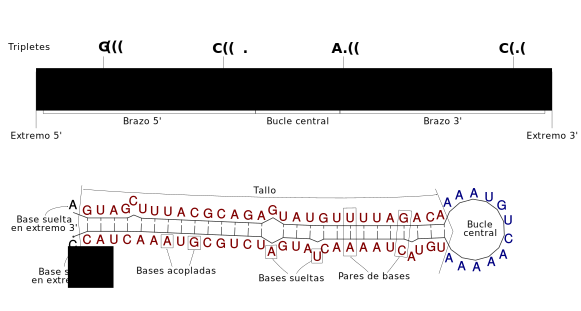
\includegraphics[width=\textwidth]{figures/triplet/triplete.pdf}

\caption{\captionStyle\protect\label{triplet}
Ejemplo de extracción de características de tripletes para el
\premirna{} \dset{cel-lsy-6}\footnotemark.
}
\end{figure}
%
El cálculo de las \caract{s} de tripletes requiere que el ejemplo
tenga una estructura secundaria con forma de horquilla, con un único
bucle central.
De otro modo, la definición del ``tallo'' pierde sentido y el
algoritmo falla, retornando valores nulos para estas \caract{s} e
invalidando cualquier procesamiento posterior del ejemplo en cuestión.
Por ello, los grupos de \caract{s} de tripletes \dset{T} y \dset{X} no
son aptos para un uso general, sino que deberán utilizarse sólo cuando
se garantice la estructura secundaria forma de horquilla para todos
los ejemplos.

En la Tabla a continuación se detallan las $36$ características de
tripletes \cite{xue} y su posición en el vector de características.

\newcommand{\tripletRow}[1]{
  \stepcounter{FeatureCounter}\theFeatureCounter & $N_{\T{\mono{#1}}}$
  & Número de ocurrencias del triplete \mono{#1} en la región del
  tallo \cite{xue}.
  }

\begin{longtable}{@{}p{0.07\textwidth}%
@{\hspace{0.01\textwidth}}p{0.17\textwidth}%
@{\hspace{0.01\textwidth}}p{0.74\textwidth}@{}}
  \headRow\endhead
  \tripletRow{A...}\\
  \tripletRow{A..(}\\
  \tripletRow{A.(.}\\
  \tripletRow{A.((}\\
  \tripletRow{A(..}\\
  \tripletRow{A(.(}\\
  \tripletRow{A((.}\\
  \tripletRow{A(((}\\
  \tripletRow{G...}\\
  \tripletRow{G..(}\\
  \tripletRow{G.(.}\\
  \tripletRow{G.((}\\
  \tripletRow{G(..}\\
  \tripletRow{G(.(}\\
  \tripletRow{G((.}\\
  \tripletRow{G(((}\\
  \tripletRow{C...}\\
  \tripletRow{C..(}\\
  \tripletRow{C.(.}\\
  \tripletRow{C.((}\\
  \tripletRow{C(..}\\
  \tripletRow{C(.(}\\
  \tripletRow{C((.}\\
  \tripletRow{C(((}\\
  \tripletRow{U...}\\
  \tripletRow{U..(}\\
  \tripletRow{U.(.}\\
  \tripletRow{U.((}\\
  \tripletRow{U(..}\\
  \tripletRow{U(.(}\\
  \tripletRow{U((.}\\
  \tripletRow{U(((}\\
  33 & $L_3$ &
  Longitud del tallo: cantidad de nucleótidos en el tallo de
  la estructura de horquilla \cite{xue}. \\
  34 & $P$ &
  Número de pares de bases en el pre-miRNA \cite{xue}. \\
  35 & $L_3/P$ &
  Grado de complementariedad entre los dos brazos de la estructura de
  horquilla: para una complementariedad perfecta, se da el valor
  mínimo 2. Este valor aumenta conforme aumenta el número de
  bases ``sueltas'' (no acopladas) en el tallo \cite{xue}. \\
  36 & $GC=\frac{N_\ntC+N_\ntG}{L_3}$ &
  Proporción de bases \ntG y \ntC en el tallo.  Se calcula contando el
  número de bases \ntC y \ntG en el tallo y dividiendo por $L_3$
  \cite{xue}.
\end{longtable}

%
%
\subsubsection{Características de la secuencia}
%
Las \caract{s} de la secuencia se proponen en los trabajos \e{miPred}
\cite{ng} y \e{microPred} \cite{batuwita}.
Se calculan directamente a partir de la cadena de texto que representa
la secuencia, ignorando las propiedades de la estructura secundaria.
Se incluyen medidas que cuentan la longitud de la secuencia, el número
de ocurrencias de las bases \ntA{}, \ntG{}, \ntC{} y \ntU{} en forma individual
y en combinaciones de dos posiciones consecutivas (dinucleótidos).
En la Tabla a continuación se enumeran las $23$ \caract{s} de la
secuencia \cite{ng,batuwita} según la posición que ocupan en el vector
de \caract{s}.

\newcommand{\dnRow}[1]{
  \stepcounter{FeatureCounter}\theFeatureCounter
  & $N_{\T{\mono{#1}}}$
  & Número de dinucleótidos \mono{#1}.}
%
\setcounter{FeatureCounter}{43}
%
\begin{longtable}{@{}p{0.07\textwidth}%
@{\hspace{0.01\textwidth}}p{0.13\textwidth}%
@{\hspace{0.01\textwidth}}p{0.78\textwidth}@{}}
  \headRow\endhead
  37 & $L$ &
  Longitud de la secuencia. \\
  38 & $N_\ntA{}$ &
  Número de nucleótidos \ntA{}. \\
  39 & $N_\ntC{}$ &
  Número de nucleótidos \ntC{}. \\
  40 & $N_\ntG{}$ &
  Número de nucleótidos \ntG{}. \\
  41 & $N_\ntU{}$ &
  Número de nucleótidos \ntU{}. \\
  42 & $N_\ntC{}+N_\ntG{}$ &
  Número de nucleótidos \ntC{} y \ntG{}. \\
  43 & $N_\ntA{}+N_\ntU{}$ &
  Número de nucleótidos \ntA{} y \ntU{}. \\
  \dnRow{AA}\\
  \dnRow{AC}\\
  \dnRow{AG}\\
  \dnRow{AU}\\
  \dnRow{CA}\\
  \dnRow{CC}\\
  \dnRow{CG}\\
  \dnRow{CU}\\
  \dnRow{GA}\\
  \dnRow{GC}\\
  \dnRow{GG}\\
  \dnRow{GU}\\
  \dnRow{UA}\\
  \dnRow{UC}\\
  \dnRow{UG}\\
  \dnRow{UU}\\
\end{longtable}

%
%
\subsubsection{Características de la estructura secundaria}
%
Al igual que las medidas de la secuencia, este grupo de \caract{s} se
basa en aquellas \caract{s} propuestas en los trabajos \e{miPred}
\cite{ng} y \e{microPred} \cite{batuwita}.
Consiste en $7$ medidas derivadas de la estructura secundaria, tales
como la ocurrencia de diferentes tipos de pares de bases (bases
acopladas) \bp{A}{U}, \bp{G}{C}, y \bp{G}{U}, y medidas basadas en un
valor denominado \e{Mínima Energía Libre}, que resulta del algoritmo
de plegado (predicción de la estructura secundaria).
A continuación, se listan las $7$ \caract{s} según la posición que
ocupan dentro del vector.

\begin{longtable}{@{}p{0.07\textwidth}%
@{\hspace{0.01\textwidth}}p{0.07\textwidth}%
@{\hspace{0.01\textwidth}}p{0.13\textwidth}%
@{\hspace{0.01\textwidth}}p{0.70\textwidth}@{}}
  \headRow\endhead
  60 & \dset{E} & MFE &
  Mínima energía libre. \\
  61 & \dset{E} & MFEI$_1$ &
  MFEI$_1=\frac{\T{MFE}}{100\cdot(N_\ntC{}+N_\ntG{})}$. \\
  62 & \dset{E} & MFEI$_4$ &
  MFEI$_4=\T{MFE}/P$. \\
  63 & \dset{E} & $dP = P/L$ &
  Número de pares de bases dividido entre la longitud total $L$. \\
  64 & \dset{E} & $P_{\bp{A}{U}}/L$ &
  Número de pares \bp{A}{U} normalizado. \\
  65 & \dset{E} & $P_{\bp{G}{C}}/L$ &
  Número de pares \bp{G}{C} normalizado. \\
  66 & \dset{E} & $P_{\bp{G}{U}}/L$ &
  Número de pares \bp{G}{U} normalizado.
\end{longtable}

%
%
%
\subsection{Normalización de los vectores de características}
%
Las \caract{s} que componen el vector de \caract{s} poseen rangos
numéricos diferentes, ya que representan cantidades de naturaleza
diversa.
Esto implica que algunos componentes del vector de \caract{s} tendrán
magnitudes mayores que otros, generando una ponderación implícita de
algunas \caract{s} por sobre otras.
La normalización permite evitar este problema modificando el rango de
cada \caract{} a un intervalo preestablecido, típicamente $[0,1]$ o
$[-1,+1]$.
Esto deriva en problemas mejor condicionados desde el punto de vista
numérico e incrementa la velocidad de convergencia en el
entrenamiento \cite{nnfaq2}.

Dado un vector de características $\xx=(x_{1},x_{2},\ldots,x_{F})$, la
versión normalizada $\xx^*$ del mismo vector se calcula según
%
\begin{align}
  \label{e3:norm-op}
  x_j^{*} = ( x_j + d_j ) s_j, \quad j=1,\ldots,F,
\end{align}
%
donde $\B{s}$ es un \e{vector de escala} y $\B{d}$ es un \e{vector de
  desplazamiento} que permiten transformar las componentes $x_j$ al
intervalo especificado.

Cuando el objetivo es la generación de un modelo de clasificador, los
vectores $\B{s}$ y $\B{d}$ se calculan con el primer archivo leído a
la entrada del método.
El primer paso es armar una matriz
$M{}_{({N}\times{}F)}$, donde cada fila $i=1,\ldots,N$ corresponde a
un ejemplo y cada columna $j=1,\ldots,\F$ representa una variable
(\caract{}).
Para cada columna $j$ de $M$, se calculan los valores $d_j$ y $s_j$
que transforman el rango de la variable $x_j$ al intervalo deseado.
Para llevar las variables al rango $[0,1]$, $d_j$ y $s_j$ se
calculan según
%
\begin{align}
  d_j &= - \min_i m_{ij}, &
  s_j &= \frac{1}{\max_i m_{ij} - \min_i m_{ij}}.
\end{align}
%
Similarmente, para llevar las variables al intervalo simétrico
$[-1,+1]$,
%
\begin{align}
  d_j &= -\frac{1}{2}\left(\max_i m_{ij} + \min_i m_{ij}\right), &
  s_j &= \frac{2}{\max_i m_{ij} - \min_i m_{ij}}.
\end{align}
%
Una vez calculados los vectores $\B{d}$ y $\B{s}$, se aplica la
normalización (\iflatexml{}Ecuación~\ref{e3:norm-op}\else\autoref{e3:norm-op}\fi)
sobre todos los ejemplos leídos en la entrada.

Para un modelo de clasificador entrenado con datos normalizados, es
importante aplicar la misma normalización sobre todos los ejemplos
futuros a clasificar.
Por ello, los vectores $\B{d}$ y $\B{s}$ se guardan como parte del
mismo modelo.
Cuando se provee un modelo como entrada al método, los ejemplos se
normalizan según la información contenida en el mismo.

%
%
%
\subsection{Partición de los datos}
%
La partición de los datos implementa el método de retención, separando
los conjuntos de datos en un conjunto \e{de entrenamiento} y otro
\e{de prueba}, a partir de la especificación del usuario al momento de
la carga de los archivos.

Internamente, los conjuntos de datos de entrenamiento y prueba se
guardan como matrices $M^E$, $M^P$, de 70 columnas y $\ell^E$ y
$\ell^P$ filas, respectivamente.
Las primeras 66 columnas representan los vectores de características
normalizados de cada ejemplo. La columna 67 contiene la clase del
ejemplo cuando es conocida. Las restantes 3 columnas contienen índices
de referencia, para lograr trazabilidad de los ejemplos.

Para cada conjunto de datos $D_n$ de $\ell_n$ elementos,
correspondiente a un archivo leído en la entrada, se arma una matriz
provisoria con los vectores de \caract{s} correspondientes a cada
ejemplo y se agrega la información de clase y los índices en las
últimas 4 columnas. Luego, se intercambian las filas en forma
pseudoaleatoria, para finalmente seleccionar las primeras
$\ell_n\cdot{}p_n^E$ filas de la matriz resultante, agregándolas al
conjunto de entrenamiento, y las $\ell_n\cdot{}p_n^P$ filas
subsiguientes al conjunto de prueba. Los valores
$0\leq{}p_n^E,p_n^P\leq1$ son especificados por el usuario e indican
la proporción de elementos del conjunto a utilizar para entrenamiento
y prueba, respectivamente.

Una vez incorporados todos los archivos en los conjuntos de
entrenamiento y prueba, se permutan sus filas en forma
pseudoaleatoria. De este modo, quedan conformados el conjunto de
entrenamiento, utilizado en la obtención del modelo, y el conjunto de
prueba, utilizado para clasificación de nuevos ejemplos.

%% Una vez efectuadas la extracción de características y la
%% normalización, los archivos de entrada originales se han convertido en
%% conjuntos $D_1,\ldots,D_N$ que contienen los vectores de
%% características normalizados y la información de clase para cada
%% ejemplo. La partición de los datos refiere al armado de los conjuntos
%% de entrenamiento $D^E$ y prueba $D^P$ con los elementos de estos
%% conjuntos a partir de la especificación del usuaio.

%% El conjunto $D_n=((\xx_i,y_i)),\,i=1,\ldots,\ell_n$ se corresponde con
%% el $n$-ésimo archivo de entrada. El objetivo es armar los conjuntos de
%% entrenamiento $D^E$ y de prueba $D^P$ con elementos de los
%% $D_n,\,n=1,\ldots,N$.  Para cada conjunto $D_n$, el usuario especifica
%% una proporción $p_n^E$ de elementos del conjunto $D_n$ a utilizar como
%% entrenamiento, y otra proporción $p_n^P$ de elementos de $D_n$ a
%% utilizar para prueba. Los valores de $p_n^E,p_n^P$ son tales que
%% %
%% \begin{align}
%%   0\ \leq\ p_n^E, p_n^P\ \leq\  p_n^E + p_n^P\ \leq\ 1,
%% \end{align}
%% %
%% esto es, $p_n^E$ y $p_n^P$ son números enre 0 y 1 cuya suma es menor o
%% igual a 1.

%% El primer paso consiste en permutar aleatoriamente el orden de los
%% elementos de los conjuntos de entrada $D_n$
%% %
%% \begin{align}
%%   D^*_n = ((\xx_j,y_j)), \quad j = \sigma(i,\ell_n,s), \quad i=1,\ldots,\ell_n,
%% \end{align}
%% %
%% donde $\sigma$ es una función de permutación pseudoaleatoria que
%% requiere la especificación de una \e{semilla} $s$. Seguidamente se
%% particiona cada conjunto $D_n$ en sub-conjuntos de entrenamiento
%% y prueba
%% %
%% \begin{align}
%%   D^E_n &= ((\xx_u,y_u)\in D^*_n),& u&=1,\ldots,\ell^E_n, \\
%%   D^P_n &= ((\xx_v,y_v)\in D^*_n),& v&=1,\ldots,\ell^P_n,
%% \end{align}
%% %
%% donde
%% %
%% \begin{align}
%%   \begin{split}
%%     \ell^E_n &= \left\lfloor\ell_n\cdot p_n^E \right\rceil, \\
%%     \ell^P_n &= \lfloor\ell_n\cdot p_n^P\rceil.
%%   \end{split}
%% \end{align}
%% %
%% El operador $\lfloor\cdot\rceil$ es el operador de redondeo.
%% Finalmente, se ensamblan los conjuntos de entrenamiento y prueba según
%% %
%% \begin{align}
%%   D^E &= \left( (\xx_u,y_u) \in \bigcup_n {D}^E_n \right), &
%%   u &= \sigma(i,\ell^E,s), &
%%   i &= 1,\ldots,\ell^E, &
%%   \ell^E &= \left| D^E \right| = \sum_n \ell^E_n ,\\
%%   D^P &= \left( (\xx_v,y_v) \in \bigcup_n {D}^P_n \right), &
%%   v &= \sigma(j,\ell^P,s), &
%%   j &= 1,\ldots,\ell^P, &
%%   \ell^P &= \left| D^P \right| = \sum_n \ell^P_n .
%% \end{align}
%% %
%% Esto es, los conjuntos de entrenamiento $D^E$ y prueba $D^P$ se arman
%% concatenando los respectivos $D^E_n$ y $D^P_n$ y luego permutando
%% aleatoriamente el orden de los ejemplos en los conjuntos resultantes.

%
%
\subsubsection{Generación de particiones para validación cruzada}
%
%La generación de las particiones de validación cruzada se lleva a cabo
%una vez armado el conjunto de entrenamiento con $\ell^E$ elementos.
Las particiones de validación cruzada se generan como un conjunto de
índices sobre el conjunto de entrenamiento.
En primer lugar, se genera un vector de índices en orden aleatorio
entre $1$ y $\ell^E$, el número de ejemplos en el conjunto de
entrenamiento.
Luego, se seleccionan los primeros $p\cdot\ell^E$ elementos para la
partición de validación, y los elementos restantes para la partición
de estimación correspondiente.
La operación se repite para cada $j=1,\ldots,k$, efectuando un
desplazamiento circular del vector de índices en $\ell^E/k$ elementos
entre iteraciones.
El parámetro $p$ regula la proporción de elementos de entrenamiento a
utilizar para validación, mientras que $k$ determina el número de
iteraciones de la validación cruzada.
Ambos parámetros pueden ser especificados por el usuario, y por
defecto se utilizan los valores $k=10$ y $p=1/k$, siguiendo el ejemplo
de la función de Matlab \func{crossval}\footnote{%
  La documentación de la función \func{crossval} puede encontrarse en
  \url{https://www.mathworks.com/help/stats/crossval.html}
}, y tal como se recomienda en \cite{hastie}.
Cuando $p=1/k$, cada ejemplo del conjunto de entrenamiento será
utilizado exactamente una vez para validación.

%
%
%
\section{Construcción del modelo del clasificador MLP}
%
La tarea de generación del modelo MLP se efectúa en dos pasos.  En
primer lugar, se determina el número óptimo de neuronas en la capa
oculta mediante una estrategia de búsqueda exhaustiva o trivial,
buscando maximizar la tasa de clasificación sobre un conjunto de
validación cruzada.

Luego se procede a efectuar el entrenamiento propiamente dicho, con
regularización de corte prematuro cuando el error de validación
cruzada alcanza su valor mínimo.

La arquitectura de la red resultante contendrá una o ninguna capa
oculta.

En todo entrenamiento del clasificador, se promedian en realidad cinco
redes inicializadas aleatoriamente, y la salida del clasificador en
realidad es un voto mayoritario de la salida de estas cinco redes.

Adicionalmente, se acepta el valor especial de 0 neuronas ocultas para
representar un MLP sin capa oculta, capaz de efectuar clasificación lineal.

Las estrategias de selección del \hparam{} de la red (el número de
neuronas en la capa oculta) son
%
\begin{description}
\item[Estrategia trivial:] Consiste en seleccionar cero neuronas
  en la capa oculta, sin entrenamiento. Esto redunda en una red que es
  capaz de efectuar separación lineal, y se utiliza como criterio de base para
  establecer el rendimiento de la red.
\item[Estrategia de búsqueda exhausiva:] Consiste en determinar, mediante prueba y error,
  el número óptimo de neuronas que maximizan una tasa promedio de validación cruzada.
\end{description}
%
Una vez encontrado el valor óptimo, se procede al entrenamiento.

%
\subsection{Estrategia trivial}
%
Tal como su nombre lo indica, esta estrategia es la más básica para
determinar el número de neuronas en la capa oculta.
Consiste simplemente en devolver siempre el valor $0$ como cantidad
``óptima'' de neuronas en la capa oculta, sin efectuar entrenamiento
alguno.
El modelo resultante al utilizar esta estrategia es equivalente a un
perceptrón simple, y funciona como un clasificador lineal.
Si bien esta estrategia no efectúa optimización alguna, resulta útil
para generar un modelo ``base'' para comparar el rendimiento frente a
otros modelos generados con una estrategia más compleja.

%
\subsubsection{Búsqueda exhaustiva}
%
La estrategia de búsqueda exhaustiva utiliza como función objetivo el
valor $G_m$ promedio de validación cruzada, y selecciona los
hiperparámetros óptimos mediante prueba y error dentro de un rango
preestablecido. Dado que la naturaleza de los hiperparámetros es
diferente según el clasificador, el algoritmo de búsqueda también
difiere en cada caso.

El hiperparámetro del perceptrón multicapa es el número de neuronas en
la capa oculta $h$, una variable discreta no negativa. La
inicialización aleatoria del perceptrón multicapa introduce
fluctuaciones aleatorias en la función objetivo $G_m$ de validación
cruzada, lo que implica que se deben efectuar una gran cantidad de
repeticiones de inicialización--entrenamiento--prueba para obtener
resultados fiables.  Por ello, en lugar de efectuar la búsqueda sobre
todos los valores posibles, se prueban 20 valores de $h$ entre 0 y 200
en una escala aproximadamente logarítmica:
%
\begin{align}
  \label{mlp-hidden-tries}
  h=0,1,2,3,4,5,7,9,11,14,19,24,32,41,54,70,91,118,154,200.
\end{align}
%
Por defecto, se efectúan 5 repeticiones de
inicialización--entrenamiento--prueba para cada valor de $h$. Se
selecciona aquel valor de $h$ para el cual se obtuvo el mayor valor de
$G_m$ de validación cruzada en promedio.

%
\subsection{Entrenamiento}
%
Una vez determinado el número óptimo de neuronas en la capa oculta,
se inicializa aleatoriamente una red MLP con la topología especificada.
Por defecto, el entrenamiento se efectúa mediante el método de
retropropagación Rprop, utilizando las rutinas propias de Matlab.
La regularización del entrenamiento se efectúa separando un 20\% de
los ejemplos, y deteniendo el entrenamiento cuando el error de
clasificación sobre estos ejemplos alcanza su valor mínimo.

La inicialización aleatoria del perceptrón multicapa condiciona el
algoritmo de retropropagación, lo que en algunos casos deriva en
soluciones subóptimas.
Para contrarrestar este efecto, se soporta el entrenamiento de
múltiples redes MLP en paralelo con inicializaciones aleatorias
diferentes.
En este caso, el modelo obtenido es en realidad un arreglo de modelos:
para obtener predicciones de clase, la salida global se determina a
partir de la \e{moda} de las salidas de los modelos contenidos en el
arreglo.

%
%
\section{Construcción del modelo del clasificador SVM}
%
AL igual que para el caso del clasificador MLP, la construcción
del modelo SVM es un proceso de dos etapas: en primer lugar se determinan
valores óptimos para los hiperparámetros, y una vez encontrados, se procede a
entrenar el modelo ``hiperparametrizado''.

A diferencia del caso MLP, sin embargo, en una máquina de vectores de soporte
los \hparam{s} pueden ser más de uno, y se trata de variables continuas.

Esto junto a las propiedades analíticas de la SVM permite aplicar estrategias
de selección de hiperparámetros más complejas que aprovechan mejor la información
del modelo SVM. Incluso, se puede aplicar optimización mediante descenso por gradiente.
%
\begin{description}
\item[Estrategia trivial:] Consiste en seleccionar hiperparámetros
  preestablecidos, sin entrenamiento. Se utiliza como estrategia
  ``básica'' para comparación de los métodos.
\item[Estrategia de búsqueda en la grilla:] Efectúa una búsqueda
  exhaustiva de los hiperparámetros maximizando la tasa de
  clasificación de validación cruzada.
\item[Estrategia de minimización del error empírico:] Realiza una
  búsqueda por gradiente en el espacio de los hiperparámetros de la
  tasa de clasificación de validación cruzada.
\item[Estrategia de minimización de la cota RMB]: Minimiza una función de derivación teórica
  intentando maximizar la tasa de clasificación.
\end{description}
%

%
%
\subsection{Selección trivial}
%
La estrategia de selección trivial consiste en seleccionar valores
preestablecidos (genéricos) para los hiperparámetros, apropiados para
la mayoría de los problemas.

La estrategia selecciona el valor $1$ para el hiperparámetro de
regularización $C$ \cite{libsvm}, y un valor $\gamma=\frac{1}{2F}$
para el hiperparámetro de amplitud del núcleo RBF, donde $F$ es el
número de características consideradas \cite{glasmachersigel}.

Es de esperar que el modelo resultante del uso de esta estrategia no
sea óptimo, aunque sí será de utilidad para la comparación con otros
modelos obtenidos mediante estrategias más avanzadas.

%
%
\subsection{Búsqueda en la grilla}
%
La \e{búsqueda en la grilla} propuesta en \cite{hsu}, permite
optimizar los hiperparámetros de regularización $C$ y $\gamma$ cuando
se utiliza un núcleo RBF.
La idea general de esta estrategia es considerar cada combinación de
hiperparámetros $(C,\gamma)$ como puntos en el plano $C\gamma$.
Comenzando por una serie de puntos espaciados regularmente
en espacio logarítmico $(\log C,\log\gamma)$, que determinan la
``grilla'' inicial, se entrena y evalúa el clasificador sobre cada
punto (cada combinación de hiperparámetros), para luego interpolar
(``refinar la grilla'') en las cercanías de los puntos donde se
obtiene la mayor tasa de clacificación $G_m$.
La búsqueda continúa repitiendo el procedimiento sobre los puntos no
evaluados hasta satisfacer un criterio de corte.

La grilla inicial viene dada por combinaciones de los siguientes
puntos de muestreo para los hiperparámetros
%
\begin{align}
  \label{initial-grid}
  \log_2 C     \tab= -5, -3, -1, 1, \ldots, 15, \tabs
  \log_2\gamma \tab= -15,-13, -11, \ldots, 3.
\end{align}
%
Para cada punto $(C_i,\gamma_j)$, se entrena y prueba el clasificador
SVM, obteniendo un ${G_m}_{ij}$ promedio de validación cruzada.

En etapas sucesivas, se interpola la grilla alrededor de los puntos
donde se obtuvieron los mejores valores $G_m$. Se definen tres
algoritmos heurísticos que determinan cuáles puntos interpolar:
%
\begin{itemize}
\item
  \e{Zoom}: En un primer paso, se convoluciona la grilla con una
  ventana cuadrada uniforme de valor unitario, obteniendo una versión
  ``suavizada'' de la grilla. Se interpolan puntos en una región
  cuadrada centrada en el punto con mayor valor $G_m$ ``suavizado''.
\item
  \e{Umbral}: A partir de un umbral $G_m$ definido por el usuario,
  por defecto el percentil 90, se interpola en cada dimensión
  alrededor de los puntos por encima del umbral.
\item
  \e{$n$-mejores}: Similar al umbral, se seleccionan $n$ puntos
  con los mayores valores de $G_m$. Se interpola la grilla en ambas
  dimensiones alrededor de estos puntos.
\end{itemize}
%
Una vez interpolada la grilla, se calcula el valor $G_m$ promedio de
validación cruzada para los puntos interpolados. El procedimiento de
refinamiento se repite hasta un máximo de $N$ iteraciones o hasta
satisfacer un criterio de corte.

La búsqueda en la grilla tiene la ventaja de ser conceptualmente
simple, sin embargo, se torna inviable cuando el vector de parámetros
$\B{\theta}$ contiene más de 2 elementos.
Dado que se trata de un método de búsqueda exhaustiva, resulta
generalmente lento.
Cuando se trabaja con un clasificador SVM con núcleo lineal, la grilla
tiene una única dimensión: la del hiperparámetro $\log C$.

%
%
\subsection{Criterio del error empírico}
%
El \e{criterio del error empírico} es una estrategia de selección de
\hparam{s} basada en la propuesta presentada en \cite{ayat}, que
optimiza los \hparam{s} del clasificador minimizando una función
objetivo denominada \e{error empírico}\,\footnote{
  El lector experto encontrará ambigua la denominación de la función
  ``error empírico'', ya que en la disciplina este nombre se utiliza
  como equivalente de ``error de entrenamiento''.
  En este trabajo, se mantiene la denominación de los autores
  \cite{ayat}, definiendo ``error empírico'' como la función que
  calcula un error probabilístico de validación cruzada sobre el
  conjunto de entrenamiento.
}.
Esta función mide el error de validación cruzada sobre el conjunto de
entrenamiento acoplando un modelo probabilístico a la salida del
clasificador, y permite su optimización mediante descenso por
gradiente ya que sus derivadas respecto de los \hparam{s} son
calculables.

En la propuesta original \cite{ayat}, la función {error empírico} se
optimiza únicamente respecto a los \hparam{s} del núcleo.
En la estrategia implementada, se agregó soporte para la optimización
del hiperparámetro $C$, siguiendo el método del cálculo de la derivada
respecto de $C$ propuesto en \cite{keerthi} y \cite{glasmachers}, tal
como se implementa en \cite{shark}.

%
\subsubsection{La función error empírico}
%
El error de validación del modelo $h$ sobre un conjunto
$V=((\xx_j,y_j))\,i=1,\ldots,\ell^V$ puede escribirse
%
\begin{align}
\label{e3:error-test-alt}
  E^V &= \frac{1}{\ell^V}\sum_{j=1}^{\ell^V} H(-{y}_j {h}(\xx_j))
\end{align}
%
donde $H(\cdot)$ es la función escalón de Heaviside. Esta formulación
del error con la función escalón $H$ en lugar de la pérdida $0-1$
equivalente pone de relieve el hecho que el error $E^V$ es una función
discontinua, al ser suma de discontinuas, y por tanto no derivable.
La función ``error empírico'' \cite{ayat} se construye a partir de una
interpretación bayesiana del concepto de error, y posee las
características deseables de continuidad y derivabilidad que permiten
su utilización como función objetivo en un esquema de minimización por
descenso por gradiente.

Si se conoce la \e{probabilidad a posteriori} $p_j$ de que el ejemplo
$\xx_j$ pertenezca a la clase positiva
%
\begin{align}
  \label{e3:pk}
  p_j = p(\xx_j) = P(h(\xx_j)=+1|\xx_j),
\end{align}
%
se puede caracterizar la \e{probabilidad de error} $E_j$ cometido al
clasificar el ejemplo $\xx_j$ según
%
\begin{align}
\label{e3:Ek}
  E_j = P(h(\xx_j)\neq y_j) = |t_j-{p}_j| =
  \begin{cases}
    {p}_j, & t_j=0\\ 1-{p}_j, & t_j = 1,
  \end{cases}
\end{align}
%
donde $t_j=\frac{y_j+1}{2}$ es un ``valor deseado'' calculado a partir
de la clase conocida $y_j$. La probabilidad de error para el conjunto
completo $V$ puede escribirse
%
\begin{align}
\label{Err1}
  E = \frac{1}{\ell^V}\sum_{j=1}^{\ell^V} E_j.
\end{align}
%
Ésta es la función \e{error empírico}. Puede comprobarse que, a
diferencia del error con pérdida 0-1, ésta es una función continua y
derivable.

Para el cálculo de $E$ se requiere conocer la probabilidad $p_j$
(\iflatexml{}Ecuación~\ref{e3:pk}\else\autoref{e3:pk}\fi), la cual no
puede determinarse a partir de la salida binaria del modelo SVM.  En
su lugar, se utiliza un estimador de $\hat{p}_j$.

%
\subsubsection{Salida probabilística del modelo SVM}
%
La salida del modelo de una máquina de vectores de soporte
(\iflatexml{}Ecuación~\ref{e2:svm-model-hard}\else\autoref{e2:svm-model-hard}\fi)
puede entenderse como el resultado de aplicar la operación signo sobre
una función continua $f$:
%
\begin{align}
\label{e3:svm-model-as-sign-f}
  h(\xx) \tab= \T{signo}(f),\tabs
  f\tab=\langle\ww,\BPhi(\xx)\rangle+b.
\end{align}
%
Aplicando el método propuesto por {Platt} en \cite{platt}, se calcula
un estimador $\hat{p}$ para la probabilidad real $p=P(h=+1|\xx)$
utilizando el valor de $f$:
%
\begin{align}
\label{e3:p-hat}
  \hat{p}\tab=\frac{1}{1+e^{Af+B}} \tabs\approx\,{}p.%P(h=+1|\xx).
\end{align}
%
Los valores $A$ y $B$ se determinan a partir del conjunto de validación
$V$ resolviendo el problema de optimización
%
\begin{align}
  \arg\min_{A,B} \tabs -\sum_{j=1}^{\ell^V} t_k\log(\hat{p}_k)+(1-t_k)\log(1-\hat{p}_k),
  \label{abproblem}
\end{align}
%
en donde $\hat{p}_k$ viene dado por la
\iflatexml{}Ecuación~\ref{e3:p-hat}\else\autoref{e3:p-hat}\fi{}, y
$t_k=\frac{1}{2}({y_k+1})$.
Este problema se resuelve mediante el algoritmo de optimización
estándar BFGS \cite{nocedal}, observando que las derivadas de
$\hat{p}_k$ respecto de $A$ y $B$ vienen dadas por
%
\begin{align}
  \begin{split}
    \dpar{\hat{p}_k}{A}{}&=-f_k e^{Af_k+B}\frac{1}{(1+e^{Af_k+B})^2}
    =-f_k\hat{p}_k(1-\hat{p}_k),\\
    \dpar{\hat{p}_k}{B}{}&=    -e^{Af_k+B}\frac{1}{(1+e^{Af_k+B})^2}
    =-   \hat{p}_k(1-\hat{p}_k).
  \end{split}
\label{e3:deriv-pk-wrt-AB}
\end{align}
%
%% Utilizando estas derivadas, el cálculo de la solución al problema
%% (\ref{abproblem}) se efectúa mediante un algoritmo de descenso por
%% gradiente.

%% La elección de una función logística como $\hat{p}_k$ se basa en la
%% presunción de que las salidas $f_k$ para las entradas $\{\xx_k\}$ de
%% clase positiva tienen una distribución gaussiana en $f$.

%% Una interpretación intuitiva de $\hat{p}_k$ es que, para una salida
%% $f_k$ de gran magnitud, que se ubica lejos del hiperplano de separación
%% en el espacio inducido por el núcleo, el clasificador SVM tiene amplia
%% certeza de su decisión.  Asimismo, se tendrá que cuando el valor de
%% $f_k=0$, $x_k$ recae exactamente en el plano de separación y se
%% obtiene la peor predicción posible $\hat{p}_k=0.5$ y, similarmente,
%% cuanto más ancho sea el margen de separación, más suave deberá ser la
%% pendiente de $\hat{p}_k$.

%
\subsubsection{Cálculo del gradiente $\grad{E}$}
\label{se:gradE}
%
Para poder utilizar un método de descenso por gradiente en el espacio
de los \hparam{s} se considera un vector genérico de \hparam{s}
$\Btheta$ de modo que $E=E(\Btheta)$, y se calculan las derivadas de
$E$ respecto de los mismos.
En primer lugar, se tiene
%
\begin{align}
\label{gradE}
  \grad{E} = \sum_{k=1}^{\ell^V} \grad{E_k} =
  \sum_{ \{i:t_k=0\}  } \grad{\hat{p}_i}
  - \sum_{ \{j:t_k=1\}  } \grad{\hat{p}_j}
  = \sum_{k=1}^{\ell^V} y_k \grad{\hat{p}_k}
\end{align}
%
Por la regla de la cadena, la derivada $\grad{\hat{p}_k}$ respecto de
un hiperparámetro ${\theta_j}$ es
%
\begin{align}
  \grad{\hat{p}_k}=\dpar{\hat{p}_k}{\theta_i}{} =
  \dpar{\hat{p}_k}{f_k}{}\dpar{f_k}{\theta_i}{} =
  -A\hat{p}_k(1-\hat{p}_k)\dpar{f_k}{\theta_i}{}.
  \label{eq:deriv-pk-thetak}
\end{align}
%
Para la determinación de $\dpar{f_k}{\theta_j}{}$ se sigue el
procedimiento propuesto en \cite{keerthi,glasmachers} e implementado
en \cite{shark}. En primer lugar, se observa que $f_k$ viene dado por
%
\begin{align}
  f_k = \langle \ww,\Phi(\xx_k)\rangle+b = \sum_{i=1}^\ell \alpha_i y_i k(\xx_i,\xx_k) + b,
  \label{fk}
\end{align}
%
en donde $((\xx_i,y_i)),i=1,\ldots,\ell$ son los ejemplos del conjunto
utilizado para entrenamiento, $k(\cdot,\cdot)$ es la función
núcleo, y $(\alpha_i, b)$ son los parámetros del modelo SVM $h$.
La derivada de $f_k$ respecto de algún hiperparámetro $\theta_j$ viene
dada por
%g
\begin{align}
  \dpar{f_k}{\theta_j}{} = \sum_{i=1}^\ell y_i
  \left[\dpar{\alpha_i}{\theta_j}{} k(\xx_i,\xx_k) + \alpha_i
    \dpar{k(\xx_i,\xx_k)}{\theta_j}{} \right].
\end{align}
%
Según sea el valor de $\alpha_i$ (el multiplicador correspondiente al
vector de entrenamiento $\xx_i$), se definen los conjuntos de índices
%
\begin{align}
  \label{unbounded-sv-set}
  u &= \left\{i\in\{1,\ldots,\ell\}:0<y_i\alpha_i<C \right\}\\
  \label{bounded-sv-set}
  g &= \left\{i\in\{1,\ldots,\ell\}: y_i\alpha_i=C \right\}\\
  n &= \left\{i\in\{1,\ldots,\ell\}: \alpha_i=0 \right\}.
\end{align}
%
Mediante interpretación geométrica de la solución al problema de la
SVM, se sabe que para aquellos vectores $\xx_i$ que no son de soporte,
se cumple que $\alpha_i=0$, luego las derivadas
$\dpar{\alpha_n}{\theta_j}{}$ son nulas. Cuando
$\alpha_i=\pm{}C$, el valor de $\alpha_g$ viene limitado (en valor absoluto) por el
parámetro $C$, y las derivadas $\dpar{\alpha_g}{\theta_j}{}$ son entonces
%
\begin{align}
  \dpar{\alpha_g}{C}{} \tab= y_g, \tabs \dpar{\alpha_g}{{\theta}^K_j}{} \tab= 0.
\end{align}
%
Aquí, $\theta_j^K$ denota un hiperparámetro específico del núcleo.
Para simplificar el cálculo de las derivadas de $\alpha_u$ y $b$ se
plantea el problema en forma matricial. Sea la \e{matriz del núcleo}
%
\begin{align}
  K = \begin{pmatrix} k(\xx_1,\xx_1) & k(\xx_1,\xx_2) & \cdots & k(\xx_1,\xx_\ell)
    \\ k(\xx_2,\xx_1) & k(\xx_2,\xx_2) & \cdots & k(\xx_2,\xx_\ell) \\ \vdots &
    \vdots & \ddots & \vdots \\ k(\xx_\ell,\xx_1) & k(\xx_\ell,\xx_2) & \cdots &
    k(\xx_\ell,\xx_\ell)
  \end{pmatrix}
  =
  \begin{pmatrix}
    (K_{uu}) & (K_{ug}) & (K_{un}) \\
    (K_{gu}) & (K_{gg}) & (K_{gn}) \\
    (K_{nu}) & (K_{ng}) & (K_{nn})
  \end{pmatrix}
\end{align}
%
donde en la matriz de la derecha los elementos de $K$ han sido
reordenados en submatrices $K_{uu},K_{ug},\ldots$ según los conjuntos
de índices $u, g, n$ definidos anteriormente.  Sea la matriz
%
\begin{align}
  H=\begin{pmatrix} K_{uu} & \B{1}_u \\ \B{1}_u^T & 0
  \end{pmatrix}
\end{align}
%
con $\B{1}_u$ un vector columna de $|u|$ elementos iguales a 1,
entonces la derivada de $(\B{\alpha}_u,b)^T$ respecto del
hiperparámetro $\theta_j$ viene dada por
%
\begin{align}
  \dpar{}{\theta^K_j}{} \begin{pmatrix}\alpha_{u}\\b\end{pmatrix} &=
    -H^{-1} \left[
      \dpar{H}{\theta^K_j}{}
      \begin{pmatrix}\alpha_{u}\\b\end{pmatrix}
        +C \begin{pmatrix}\dpar{K_{gu}}{\theta^K_j}{}\\0\end{pmatrix}
          y_g
          \right], \\
  \dpar{}{C}{} \begin{pmatrix}\alpha_{u}\\b\end{pmatrix} &=
    -H^{-1} \left[
      \begin{pmatrix}{K_{gu}}\\\B{1_g^T}\end{pmatrix} y_g
      \right],
\end{align}
%
donde $\B{1}_g$ un vector columna de $|g|$ elementos iguales a 1 y
$\B{y}_g$ el vector de clases correspondientes a los elementos en
$g$. Para los detalles de este resultado se refiere al lector a
\cite{glasmachers} y \cite{keerthi}.

Una vez obtenidas las derivadas de $({\B{\alpha},b})^T$ respecto de
los hiperparámetros $\B{\theta}$, la derivada de $f$  respecto
de los mismos se calcula simplemente según
%
\begin{align}
  \dpar{f_k}{C}{} &=  \sum_{i=1}^l y_i\left[
    \dpar{\alpha_i}{C}{} k(x_i,x_k) \right]
  + \dpar{b}{C}{} ,\\
  \dpar{f_k}{\theta^K_j}{} &=  \sum_{i=1}^l y_i \left[
    \dpar{\alpha_i}{\theta^K_j}{} k(x_i,x_k) +
    \dpar{k(x_i,x_k)}{\theta^K_j}{} \alpha_i \right]
  + \dpar{b}{\theta^K_j}{}.
\end{align}
%
Reemplazando estos resultados en (\ref{eq:deriv-pk-thetak}), el cálculo
del gradiente $\nabla{}E$ (\ref{gradE}) se efectúa directamente.

%
\subsubsection{Algoritmo de optimización}
%
El algoritmo comienza la búsqueda estableciendo en $1$ el valor de
todos los \hparam{s}: $\Btheta^0=(1,1,\ldots)$.
En cada iteración $t$, se efectúan los siguientes pasos:
%
\begin{enumerate}
\item
  Aplicando validación cruzada, se entrena un modelo SVM para cada
  conjunto de estimación.
\item
  Se calculan las salidas $f_k$
  (\iflatexml{}Ecuación~\ref{fk}\else\autoref{fk}\fi) de los modelos
  para todos los ejemplos $\xx_k$ en las respectivas particiones de
  validación.
\item
  Se determinan los valores óptimos de los parámetros $A$ y $B$,
  minimizando el Problema~\ref{abproblem}, partiendo de los valores
  iniciales $A_0=1$, $B_0=0$.
\item
  Se calculan las probabilidades estimadas $\hat{p}_k$ y con ellas, el
  error empírico de cada ejemplo $E_k$ y global $E$.
\item
  Se calculan las derivadas $\dpar{E}{\theta_j}{}$.
\end{enumerate}
%
La búsqueda procede en cada punto $\Btheta^t$ evaluando la función
objetivo $E$ y determinando un nuevo punto $\Btheta^{t+1}$ a partir de
la información disponible en el gradiente $\nabla{}E^t$, mediante el
algoritmo de optimización BFGS \cite{nocedal}.

%
%
\subsection{Minimización de la cota radio-margen}
%
Una cota ``radio-margen'' es una función de derivación teórica que
sirve como límite superior al error de clasificación
\e{dejando-uno-fuera} del modelo SVM sobre el conjunto de
entrenamiento.
La primera función de este tipo fue propuesta en \cite{vapnik}
para modelos SVM con regularización $L2$ y viene dada por
% vapnik sec. 10.7, pag 441
\begin{align}
  \T{RM} = 4R^2 \|\ww\|^2.
\end{align}
%
Aquí, $R$ es el radio de la hiperesfera que contiene todos los
vectores de soporte en el espacio inducido $Z$ y $\ww$ es el vector
normal al hiperplano de separación del modelo.
Puede mostrarse que la función RM cumple la propiedad
%
\begin{align}
  E_{\T{LOO}} \leq \T{RM},
\end{align}
%
donde $E_{\T{LOO}}$ es el error de validación cruzada dejando uno
fuera.
Esta propiedad, junto al hecho de ser derivable respecto de los
\hparam{s}, convierte a RM en una función objetivo idónea en un
esquema de minimización mediante descenso por gradiente.
En \cite{chapelle} se presenta un método para selección automática de
hiperparámetros basado en esta función.
Sin embargo, su utilidad práctica es limitada, ya que
la SVM con regularización $L2$ no es muy utilizada.

En \cite{chung} se proponen formulaciones alternativas a RM,
aplicables a una formulación SVM con regularización $L1$ y núcleo
gaussiano (RBF).
En particular, se considera la función
%
\begin{align}
  \rho = \rho_R \cdot \rho_M,
\end{align}
%
donde $\rho_R$ y $\rho_M$ son, respectivamente, los factores ``radio''
y ``margen''
%
\begin{align}
  \rho_R &= R^2+\frac{1}{C}, \\
  \rho_M &= \|\ww\|^2+2C\sum\xi_i.
\end{align}
%
A diferencia de {RM}, la función $\rho$ ajusta el error $E_{\T{LOO}}$
con demasiada holgura, por lo que pierde el significado original de
representar una tasa de error.
Sin embargo, mantiene la propiedad de poseer un mínimo global cerca
del punto que minimiza la tasa de error $E_{\T{LOO}}$.

\subsubsection{Función objetivo}
La estrategia aquí propuesta utiliza una de estas cotas
alternativas, denotada $\rho$ y definida según

\begin{align}
  \rho = \rho_R \cdot \rho_M,
\end{align}
donde $\rho_R$, $\rho_M$ son los factores ``radio'' y ``margen''

\begin{align}
  \rho_R &= R^2+\frac{1}{C}, \\
  \rho_M &= \|\ww\|^2+2C\sum\xi_i.
\end{align}
A diferencia de $\T{RM}$, la función $\rho$ ajusta el valor
real de $E_{\T{LOO}}$ con demasiada holgura, con lo que su valor
pierde el significado original de representar una tasa de error. Sin
embargo, tiene la importante propiedad de poseer un mínimo global en
las cercanías de los hiperparámetros óptimos $(C,\gamma)$ que
minimizan la tasa de error $E_{\T{LOO}}$.

\subsubsection{Cálculo de $\rho$}
El valor $R^2$, necesario para el cálculo de $\rho_R$, viene dado por

\begin{align}
  R^2 = 1 - \Bbeta_*^T \KK \Bbeta_*,
\end{align}
donde $\Bbeta_*$ es la solución al problema de optimización conocido
como ``SVM de una clase'' \cite{scholkopf}

\begin{align}
\begin{split}
  \arg\min_{\Bbeta}\quad&\Bbeta^T \KK \Bbeta,\\
  \T{sujeto a}    \quad&0\leq\beta_i\leq{}1,\quad{}i=1,\ldots,\ell,\\
                       &\B{1}^T_\ell\,\Bbeta=1.
  \end{split}
  \label{svm-oneclass}
\end{align}
Aquí, $\B{1}_{\ell}$ es un vector columna con $\ell$ elementos iguales
a 1, y $\KK$ es la matriz del núcleo con elementos
$k_{ij}=k(\xx_i,\xx_j)$. La matriz $\KK$ es definida positiva siempre
que se cumpla la condición

\begin{align}
\label{cond-kmatrix-defpos}
  i\neq j \iff \xx_i\neq\xx_j,\quad \forall\,i,j\in{1,\ldots,\ell},
\end{align}
esto es, siempre que no haya ejemplos repetidos en el conjunto de
entrenamiento. Sin perder mucha generalidad, se considera que tal es
el caso, y con ello, se asegura que el problema \cite{svm-oneclass}
tiene solución única \cite{SOL-UNICA-DEFINIDA-POSITIVA}.

El valor ``margen'' $\rho_M$ es dos veces la solución al problema de
optimización de la SVM (\autoref{svm-primal-blando}).  Dada la
equivalencia primal-dual de la solución, si $\Balpha$ es solución a
la forma dual (\autoref{svmprob-dual-soft}), se tiene simplemente

\begin{align}
\label{prieqdual}
  \rho_M &= 2\left(\frac{1}{2}\|\ww\|^2+C\sum\xi_i \right)
  =2\left(\B{e}^T\Balpha-\frac{1}{2}\Balpha^T\B{Q}\Balpha\right),
\end{align}
donde $\QQ$ es la matriz con elementos $Q_{ij}=y_iy_jk(\xx_i,\xx_j)$.

%
\subsubsection{Cáclulo del gradiente $\nabla\rho$}
%
El cálculo de las derivadas de $\rho$ se basa en resultados de
análisis de perturbación de problemas de optimización, ya que tanto
$\rho_R$ como $\rho_M$ son soluciones a problemas de este tipo
\cite{chung}.
Las derivadas de $\rho_R$ respecto de los hiperparámetros $C$ y
$\gamma$ vienen dadas por
%
\begin{align}
%
  \dpar{\rho_R}{C}{} &
  = \dpar{}{C}{}\left(1-\Bbeta^T\KK\Bbeta\right)
       + \dpar{}{C}{}\left(\frac{1}{C}\right)
  = -\Bbeta^T \dpar{\KK}{C}{}\Bbeta - \frac{1}{C^2}
  = -\frac{1}{C^2}, \\[1ex]
%
  \dpar{\rho_R}{\gamma}{} &
  = \dpar{}{\gamma}{}\left(1-\Bbeta^T\KK\Bbeta)\right)
       + \dpar{}{\gamma}{}\left(\frac{1}{C}\right)
  = -\Bbeta^T \dpar{\KK}{\gamma}{}\Bbeta.
%
\end{align}
%
Para garantizar la existencia de estas derivadas, resulta necesario
reescribir las restricciones $\alpha_i\leq{}C$ del problema de la SVM
(\ref{svmprob-dual-soft}) de forma tal que las mismas no dependan del
\hparam{} $C$ \cite{chung}.
Esto se logra efectuando el cambio de variable
$\bar{\Balpha}=\Balpha/C$ en (\ref{svmprob-dual-soft}):
%
\begin{align}
\begin{split}
    \max_{\bar{\Balpha}}\quad&
    f(\bar{\Balpha}) = C^2 \left( \frac{\B{1}^T\bar{\Balpha}}{C}
    -\frac{1}{2}\bar{\Balpha}^T\QQ\bar{\Balpha}\right)\\
    \T{sujeto a}\quad & \yy^T\bar{\Balpha} = 0, \\
    & 0\leq\bar{\alpha}_i\leq 1,
    \T{ para todo } i\in {1,\ldots,\ell }.
\end{split}
\end{align}
%
Con este cambio de variable el valor de $\rho_M$ viene dado por:
%
\begin{align}
  \label{eq:rmb-alpha-equiv}
  \rho_M=2\left(\B{e}^T\Balpha-\frac{1}{2}\Balpha^T\B{Q}\Balpha\right)
  = 2C^2\left(\frac{\B{1}^T\bar{\Balpha}}{C} -
  \frac{1}{2}\bar{\Balpha}^T\QQ\bar{\Balpha}\right).
\end{align}
%

Las derivadas de $\rho_M$ respecto a los \hparam{s} $C$ y $\gamma$ se
calculan según:
%
\begin{align}
    \dpar{\rho_M}{C}{}
    &= \dpar{}{C}{}\left( 2C^2\left(\frac{\B{1}^T\bar{\Balpha}}{C} -
    \frac{1}{2}\bar{\Balpha}^T\QQ\bar{\Balpha}\right)
    \right) \nonumber\\
    &= 4C \left(\frac{\B{1}^T\bar{\Balpha}}{C} -
    \frac{1}{2}\bar{\Balpha}^T\QQ\bar{\Balpha}\right)
    - 2C^2 \left(\frac{\B{1}^T\bar{\Balpha}}{C^2} \right) \nonumber\\
    &= 2\left(\B{1}^T\bar{\Balpha}
    - C \bar{\Balpha}^T\QQ\bar{\Balpha}\right) \nonumber\\
    &= \frac{2}{C} \left(\B{1}^T\Balpha - \Balpha^T\QQ\Balpha\right),\\[1ex]
    \dpar{\rho_M}{\gamma}{}
    &= \dpar{}{\gamma}{}
    2\left(  \B{1}^T\Balpha-\frac{1}{2}\Balpha^T\QQ\Balpha \right) \nonumber\\
    &= - \Balpha^T \dpar{\QQ}{\gamma}{}\Balpha \nonumber\\
    & = - \Balpha^T \left(\yy^T \dpar{\KK}{\gamma}{}\yy\right) \Balpha.
    %% \\
    %% & = \sum_{i,j=1}^\ell \alpha_i\alpha_j y_i y_j \dpar{k(\xx_i,\xx_j)}{\gamma}{}, \\[0.2em]
\end{align}
%
Los elementos $\dpar{k_{ij}}{\gamma}{}$ de la matriz
$\dpar{\KK}{\gamma}{}$ vienen dados por
%
\begin{align}
  \dpar{k_{ij}}{\gamma}{}
  = \dpar{}{\gamma}{}k(\xx_i,\xx_j)
  = \dpar{}{\gamma}{} \left(e^{-\gamma\|\xx_i-\xx_j\|}\right)
  = -k_{ij}\|\xx_i-\xx_j\|.
\end{align}
%
Finalmente se calculan las derivadas de $\rho$ respecto de $C$ y
$\gamma$ mediante
%
\begin{align}
    \dpar{\rho}{C}{} &= \dpar{\rho_M}{C}{} \rho_R + \rho_M \dpar{\rho_R}{C}{} \nonumber\\
    &= \frac{2}{C} \left(\B{1}^T\Balpha - \Balpha^T\QQ\Balpha\right) \left( R^2 + \frac{1}{C} \right)
    - 2\left(  \B{1}^T\Balpha-\frac{1}{2}\Balpha^T\QQ\Balpha \right)
    \left( \frac{1}{C^2} \right) \label{drho-dc}, \\[1em]
    \dpar{\rho}{\gamma}{} &= \dpar{\rho_M}{\gamma}{} \rho_R + \rho_M \dpar{\rho_R}{\gamma}{}\nonumber\\
    &= \left( - \Balpha^T \left(\yy^T \dpar{\KK}{\gamma}{}\yy\right) \Balpha \right)
    \left( R^2 + \frac{1}{C} \right)
    - 2\left(  \B{1}^T\Balpha-\frac{1}{2}\Balpha^T\QQ\Balpha \right)
    \left( \Bbeta^T \dpar{\KK}{\gamma}{} \Bbeta \right), \label{drho-dgamma}
\end{align}
%
en donde los elementos de las matrices $\QQ$ y $\dpar{\KK}{\gamma}{}$
son
%
\begin{align}
  q_{ij}&=y_i y_j k(\xx_i,\xx_j)= y_i y_j e^{-\gamma\|\xx_i-\xx_j\|}, \\
  \dpar{k_{ij}}{\gamma}{}&=-k_{ij}\|\xx_i-\xx_j\| = -\|\xx_i-\xx_j\|e^{-\gamma\|\xx_i-\xx_j\|}.
\end{align}
%

%
\subsubsection{Algoritmo de optimización}
%
Partiendo de un punto inicial $(C^0,\gamma^0)$ la búsqueda procede
en cada punto $(C^k,\gamma^k)$ evaluando $\rho^k$ y determinando
un nuevo punto $(C^{k+1},\gamma^{k+1})$ en la dirección del
negativo del gradiente $\nabla\rho^k$ tal que $\rho^{k+1}<\rho^k$.
La optimización de la función $\rho$ se efectúa mediante el algoritmo
BFGS \cite{nocedal} en el espacio logarítmico de los hiperparámetros
$(\ln(C),\ln(\gamma))$.
Este cambio de coordenadas se traduce en un incremento de la
estabilidad numérica y evita tener que verificar en cada iteración la
no-negatividad de $C$ y $\gamma$.
%
\begin{align}
  \dpar{\rho}{\ln C}{}= C \dpar{\rho}{C}{}, &&
  \dpar{\rho}{\ln \gamma}{}= \gamma \dpar{\rho}{\gamma}{}
\end{align}
%
Para un conjunto de entrenamiento $D=((\xx_i,y_i),i=1,\ldots,\ell)$
cada evaluación de $\rho(\Btheta_k)$ consta de los siguientes pasos
%
\begin{enumerate}
\item Entrenar una máquina de vectores de soporte con núcleo RBF
  con hiperparámetros $\Btheta_k=(C_k,\gamma_k)$ sobre el conjunto
  de entrenamiento completo $D$
\item Calcular $\Bbeta_*$ óptimo para el problema (\ref{svm-oneclass})
\item Calcular el valor de $\rho$ como el producto de
  $\rho_M$ (\ref{rho_m}) y $\rho_r$ según (\ref{rho_r})
\item Calcular el gradiente $\nabla\rho$.
\end{enumerate}
%


%
%
\subsection{Entrenamiento}
%
Una vez determinados los \hparam{s} del clasificador mediante alguna
de las estrategias antes definidas, se entrena el modelo SVM ``final''
a partir del conjunto de entrenamiento $D$ generado en la etapa de
preprocesamiento.
El modelo entrenado incorpora toda la información necesaria para poder
clasificar nuevos ejemplos, incluyendo la información de normalización
extraída del conjunto de entrenamiento.
Esto permite además la utilización del modelo como entrada al
preprocesamiento para normalizar los nuevos ejemplos a clasificar.

%
%
%
\section{Clasificación}
%
Cuando el objetivo es obtener predicciones de clase, el método recibe
como entrada un modelo de clasificador $h$ y un conjunto de datos de
prueba $T$.
La clasificación se efectúa invocando la función apropiada para el
modelo en cuestión, pasándole como argumento el conjunto de datos de
prueba leído.
La salida es un vector ${\yy}=(\hat{y}_1,\hat{y}_2,\ldots)^T$, que
contiene las predicciones de clase $\hat{y}_i$ correspondientes a cada
ejemplo $\xx_i$ del conjunto $T$:
%
\begin{align*}
  \hat{y}_i &= h(\xx_i), & \xx_i&\in{}T.
\end{align*}
%

%
%
%
\section{Interfaz de usuario}
%
El sistema incluye una interfaz de usuario de línea de comandos de
``alto nivel'', común para los distintos tipos de clasificadores
soportados.
Esta interfaz de usuario consiste en tres funciones específicas que
permiten al usuario cargar los datos del disco, generar el modelo del
clasificador, y clasificar nuevos datos.
%
\begin{enumerate}
\item
  La función \func{problem\_gen} carga datos de entrenamiento y de
  prueba según la especificación del usuario, y retorna una estructura
  en memoria denominada ``problema'', que puede utilizarse como
  entrada a las funciones de obtención del modelo y de clasificación.
  A grandes rasgos, esta función lleva a cabo la etapa de
  preprocesamiento de los datos.
\item
  La función \func{select\_model} permite obtener el modelo del
  clasificador a partir de los datos de entrenamiento.
  Recibe como argumento un problema generado con \func{problem\_gen},
  y retorna un modelo de clasificador óptimo según las opciones
  especificadas como parámetros.
  La función ofrece la funcionalidad de construcción del modelo del
  clasificador tanto MLP como SVM, con sus respectivas estrategias de
  selección de hiperparámetros.
\item
  La función \func{problem\_classify} permite clasificar los datos de
  prueba especificados dentro de un problema generado con
  \func{problem\_gen}.
  Recibe como argumento el modelo entrenado y el problema que se desea
  clasificar, y retorna una estructura en memoria con las predicciones
  para todos los elementos incluidos en el conjunto de prueba
  definidos en el problema.
\end{enumerate}
%
Los casos de uso típicos del sistema son la generación de un modelo de
clasificador y la obtención de predicciones de clase.
Utilizando las funciones de interfaz de usuario, estas tareas pueden
efectuarse según los siguientes pasos
\begin{itemize}
\item
  Obtener un nuevo modelo de clasificador:
  %
  \begin{enumerate}
  \item
    Generar un problema de clasificación mediante la función
    \func{problem\_gen} que contenga datos de entrenamiento de clase
    positiva así como negativa.
  \item
    Entrenar un clasificador invocando a la función
    \func{select\_model}.
  \end{enumerate}
  %
\item
  Obtener predicciones de clase:
  %
  \begin{enumerate}
  \item
    Generar un problema de clasificación mediante la función
    \func{problem\_gen} que contenga datos de prueba para clasificar.
  \item
    Invocar la función \func{problem\_classify}, pasándole como
    argumentos el problema y un modelo obtenido mediante
    \func{select\_model}.
  \end{enumerate}
  %
\end{itemize}
%

%
%
\section{Web de demostración del clasificador}
%
Se generó una interfaz web de demostración utilizando la herramienta
\eng{\webdemo{}} \cite{webdemobuilder}, que interactúa con el
clasificador a través de una función codificada a tal fin.
Esta función recibe un número de argumentos fijos, que son presentados
como campos del formulario web, y luego de ser invocada retorna un
``reporte'' que se presenta al usuario.
Cuando la invocación es exitosa, el reporte contiene el modelo
generado y las predicciones de clase del conjunto de prueba (si
corresponde), y puede descargarse y utilizarse posteriormente como
modelo para clasificar nuevos datos.
Cuando se encuentran errores, el reporte informa al usuario del
problema ocurrido.

%% Los argumentos de entrada en el formulario web son:
%% %
%% \begin{enumerate}
%% \item Tipo de clasificador requerido
%% \item Grupos de \caract{s} a incluir
%% \item Estrategia de selección de \hparam{s}
%% \item Archivo con datos de entrenamiento de clase positiva
%% \item Archivo con datos de entrenamiento de clase negativa
%% \item Modelo generado previamente
%% \item Archivo con datos de prueba
%% \item Clase de los datos de prueba (usado para estadísticas)
%% \end{enumerate}
%% %
Según la tarea que desee efectuar, el usuario debe cargar/seleccionar
los siguientes datos en el formulario web:
%
\begin{itemize}
\item
  {Para la generación del modelo del clasificador}:
  %
  \begin{itemize}
  \item
    Tipo de clasificador
  \item
    Conjunto de características
  \item
    Estrategia de selección de \hparam{s}
  \item
    Archivo FASTA con datos de entrenamiento de clase positiva
  \item
    Archivo FASTA con datos de entrenamiento de clase negativa
  \end{itemize}
  %
\item
  {Para efectuar clasificación con un modelo generado previamente}:
  %
  \begin{itemize}
  \item
    Archivo con el modelo de clasificador
  \item
    Archivo FASTA con datos de prueba
  \item
    Clase de los datos de prueba: opcional, utilizado para calcular
    una tasa de error sobre el conjunto.
  \end{itemize}
  %
\end{itemize}
%
Luego de la ejecución, se muestra en pantalla un enlace al archivo de
reporte, que puede ser descargado y almacenado para su utilización
posterior.

%
%\subsection{Publicación de la interfaz web de demostración}
%
\paragraph{Puesta en servicio de la demostración web}
\pdfcomment[color=Orange,open=true]{
  La idea es describir aquí la puesta en servicio de la web-demo.
}

%
%
\section{Documentación}
%
Se redactó una una guía del usuario que detalla las instrucciones de
instalación, los requerimientos del sistema, la utilización de la
interfaz de línea de comandos, y la generación y utilización de la
interfaz web.
La guía del usuario puede consultarse en el
\iflatexml{}Anexo~\ref{guiausuario}\else\autoref{guiausuario}\fi de
este documento.

Además de la guía de usuario, se incorporaron unas 700 líneas de
documentación en el código fuente siguiendo el estándar de
documentación de Matlab, lo que permite su consulta en línea mediante
la función nativa \func{help}.

\renewcommand{\bibfont}{\normalfont\footnotesize}
\printbibliography
\end{document}

